\chapter{Zero density energy theorems}\label{zero-density-energy-chapter}


\begin{definition}[Zero density exponents]\label{zeroe-def}  For $1/2 \leq \sigma \leq 1$ and $T>0$, let $N^*(\sigma,T)$ denote the additive energy $E_1(\Sigma)$ of the imaginary parts of the zeroes $\rho$ of the Riemann zeta function with $\mathrm{Re}(\rho) \geq \sigma$ and $|\mathrm{Im}(\rho)| \leq T$.  For fixed $1/2 \leq \sigma \leq 1$, the zero density exponent $A^*(\sigma) \in [-\infty,\infty)$ is the infimum of all exponents $\A^*$ for which one has
    $$ N^*(\sigma-\delta,T) \ll T^{A^* (1-\sigma)+o(1)}$$
for all unbounded $T$ and infinitesimal $\delta>0$.
\end{definition}

The exponent $\A^*(\sigma)$ is also essentially referred to as $B(\sigma)$ in \cite{heath_brown_consecutive_II} (though without the technical shift by $\delta$ in that reference).

\python{zero_density_energy_estimate}
\code{Zero_Density_Energy_Estimate}

\begin{lemma}[Basic properties of $\A^*$]\label{zeroe-basic}\uses{zeroe-def}\
\begin{itemize}
\item[(i)] We have the trivial bounds
$$ 2\A(\sigma), 4\A(\sigma)-\frac{1}{1-\sigma} \leq \A^*(\sigma) \leq 3 \A(\sigma)$$
for any $1/2 \leq \sigma \leq 1$.
\item[(ii)] $\sigma \mapsto (1-\sigma) \A^*(\sigma)$ is non-increasing, with $\A^*(1/2)=6$ and $\A^*(1)=-\infty$.
\item[(iii)] If the Riemann hypothesis holds, then $\A^*(\sigma)=-\infty$ for all $1/2 < \sigma \leq 1$.
\end{itemize}
\end{lemma}

\python{zero_density_energy_estimate}
\code{add_trivial_zero_density_energy_estimates(hypotheses)}

\begin{proof}\uses{add-energy, zero-basic} The claim (i) follows from Lemma \ref{add-energy}(iv), and the remaining claims then follow from Lemma \ref{zero-basic}.\end{proof}

Upper bounds on $\A^*(\sigma)$ can be obtained from large value energy theorems via the following relation.

\begin{lemma}[Zero density energy from large values energy]\label{zeroe-from-large}\uses{lvze-def}  Let $1/2 < \sigma < 1$.  Then
$$ \A^*(\sigma)(1-\sigma) \leq \max\left( \sup_{\tau \geq 1} \LV^*_\zeta(\sigma,\tau)/\tau, \limsup_{\tau \to \infty} \LV^*(\sigma,\tau)/\tau \right).$$
\end{lemma}

\begin{proof}\uses{lve-basic,zero-from-large,add-energy, lve-asymp}
Write the right-hand side as $B$, then $B \geq 0$ (from Lemma \ref{lve-basic}(iii)) and we have
\begin{equation}\label{lvze-bound}
    \LV^*_\zeta(\sigma,\tau) \leq B \tau
\end{equation}
for all $\tau \geq 1$, and
\begin{equation}\label{lve-bound}
    \LV^*(\sigma,\tau) \leq (B+\eps) \tau
\end{equation}
whenever $\eps>0$ and $\tau$ is sufficiently large depending on $\eps$ (and $\sigma$).  It would suffice to show, for any $\eps>0$, that $N^*(\sigma,T) \ll T^{B+O(\eps)+o(1)}$ as $T \to \infty$.

By dyadic decomposition, it suffices to show for large $T$ that the additive energy of imaginary parts of zeroes in $[T,2T]$ is $\ll T^{B+O(\eps)+o(1)}$.  As in the proof of Lemma \ref{zero-from-large}, we can assume the imaginary parts are $1$-separated (here we take advantage of the triangle inequality in Lemma \ref{add-energy}(iii)).

Suppose that one has a zero $\sigma'+i t$ of this form.  Then by standard approximations to the zeta function, one has
$$ \sum_{n \leq T} \frac{1}{n^{\sigma'+it}} \ll T^{-1}.$$
Let $0 < \delta_1 < \eps$ be a small quantity (independent of $T$) to be chosen later, and let $0 < \delta_2 < \delta_1$ be sufficiently small depending on $\delta_1,\delta_2$.  By the triangle inequality, and refining the sequence $t'$ by a factor of at most $2$, we either have
$$ \bigg|\sum_{T^{\delta_1} \leq n \leq T} \frac{1}{n^{\sigma'+it}} \bigg| \gg T^{-\delta_2}$$
for all zeroes, or \eqref{td}
for all zeroes.

Suppose we are in the former (``Type I'') case, we can dyadically partition and conclude from the pigeonhole principle that
$$ \bigg| \sum_{n \in I} \frac{1}{n^{\sigma'+it}} \bigg| \gg T^{-\delta_2-o(1)}$$
for some interval $I$ in some $[N,2N]$ with $T^{\delta_1} \ll N \ll T$, with at most $O(\log T)$ different choices for $I$.  Performing a Fourier expansion of $n^{\sigma'}$ in $\log n$ and using the triangle inequality one can then deduce that
$$ \bigg| \sum_{n \in I} \frac{1}{n^{it'}} \bigg| \gg N^{\sigma'} T^{-\delta_2-o(1)}$$
for some $t' = t + O(T^{o(1)})$; refining the $t$ by a factor of $T^{o(1)}$ if necessary, we may assume that the $t'$ are $1$-separated and that the interval $I$ is independent of $t'$, and by passing to a subsequence we may assume that $T = N^{\tau+o(1)}$ for some $1 \leq \tau \leq 1/\delta_1$, then
$$ \bigg| \sum_{n \in I} \frac{1}{n^{it'}} \bigg| \gg N^{\sigma-\delta_2/\delta_1+o(1)}$$
for all $t'$.  If we let $\Sigma'$ denote the set of such $t'$, then by Definition \ref{lvze-def} we then have (for $\delta_2$ small enough) we have
$$ E_1(\Sigma') \ll N^{\LV^*_\zeta(\sigma,\tau) + \eps + o(1)} \ll T^{\LV^*_\zeta(\sigma,\tau)/\tau + \eps + o(1)}.$$
By Lemma \ref{add-energy}(i) this implies that the set $\Sigma$ of real parts of zeroes under consideration also obeys the bound
$$ E_1(\Sigma) \ll T^{\LV^*_\zeta(\sigma,\tau)/\tau + \eps + o(1)}.$$
and the claim follows in this case from \eqref{lvze-bound}.

The Type II case similarly follows from \eqref{lve-bound} exactly as in the proof of Lemma \ref{zero-from-large}.
\end{proof}


\begin{corollary}\label{zeroe-large-cor-0}\uses{zeroe-def, lvze-def} Let $1/2 < \sigma < 1$ and $\tau_0 > 0$ be fixed.  Then
$$ \A^*(\sigma)(1-\sigma) \leq \max \left(\sup_{2 \leq \tau < \tau_0} \LV^*_\zeta(\sigma,\tau)/\tau, \sup_{\tau_0 \leq \tau \leq 2\tau_0} \LV^*(\sigma,\tau)/\tau\right)$$
\end{corollary}

\python{zero_density_energy_estimate}
\code{lver_to_energy_bound(LVER, LVER_zeta, sigma_interval)}

\begin{proof}  Repeat the proof of Corollary \ref{zero-large-cor-0}.
\end{proof}

\section{Known additive energy bounds}

\begin{proposition}[Additive energy under the Lindelof hypothesis]\label{zeroe-lindelof}\uses{zeroe-def}  Let $1/2 \leq \sigma \leq 1$ be fixed.  Then one has
    $$ \A^*(\sigma) \leq 8 - 4\sigma$$
    and $\A^*(\sigma) \leq 0$ if $\sigma > 3/4$.
\end{proposition}

\begin{proof} See \cite[Lemma 4]{heath_brown_consecutive_II}.
\end{proof}

\begin{theorem}[Heath-Brown's additive energy bound]\label{hb-energy-bound}\cite[Theorem 2]{heathbrown_zero_1979}\uses{zeroe-def}  Let $1/2 \leq \sigma \leq 1$ be fixed.  Then one can bound $A^*(\sigma)$ by
    \begin{align*}
        \frac{10-11\sigma}{(2-\sigma)(1-\sigma)} & \hbox{ for } 1/2 \leq \sigma \leq 2/3;\\
        \frac{18-19\sigma}{(4-2\sigma)(1-\sigma)} & \hbox{ for } 2/3 \leq \sigma \leq 3/4;\\
        \frac{12}{4\sigma-1} & \hbox{ for } 3/4 \leq \sigma \leq 1.
    \end{align*}
\end{theorem}

\literature
\code{add_zero_density_energy_heath_brown_1979()}
\derived
\code{prove_heath_brown_energy_estimate()}

\begin{proof}\uses{zeroe-large-cor-0, power-energy, hb-energy-simp, l2-mvt, hb-density, zeroe-basic, lvz-basic} We first suppose that $\sigma \leq 3/4$.  Here we apply Corollary \ref{zeroe-large-cor-0} with $\tau_0 = 2$.  The $\LV^*_\zeta$ supremum is now trivial, so it suffices to show that
\begin{equation}\label{second-claim}
        \rho^* \leq \max\left( \frac{10-11\sigma}{2-\sigma}, \frac{18-19\sigma}{4-2\sigma}\right) \tau
\end{equation}
whenever $(\sigma,\tau,\rho,\rho^*,s) \in \Energy$ with $2 \leq \tau \leq 3$.  Let $k$ be the first integer for which $1 \leq \tau/k \leq 3/2$, thus $k=2,3$ and also $\tau/(k+1) \leq 1$.  By Lemma \ref{power-energy}, there exist tuples
\begin{equation}\label{smak}
\left(\sigma, \frac{\tau}{k}, \rho', \frac{\rho^*}{k}, s'\right), \left(\sigma,\frac{\tau}{k+1}, \rho'', \frac{\rho^*}{k + 1}, s''\right)  \in \Energy.
\end{equation}
for some $\rho'$, $s'$, $\rho''$ and $s''$ satisfying
\[
\rho' \le \frac{\rho}{k},\qquad s' \le \frac{s}{k},\qquad \rho'' \le \frac{\rho}{k+1},\qquad s'' \le \frac{s}{k+1}.
\]
Applying Corollary \ref{hb-energy-simp} to the former tuple of \eqref{smak} and using $\rho' \le \rho/k$, we have
$$\frac{\rho^*}{k} \leq \max \left(\frac{3\rho}{k} + 1-2\sigma, \frac{\rho}{k} +4-4\sigma, \frac{5\rho}{2k} + \frac{3-4\sigma}{2}\right).$$
Write $\tau' := \tau/k$. Applying Lemma \ref{l2-mvt} to the first tuple of \eqref{smak} one has
$$\rho/k \leq \tau' + 1 - 2\sigma$$
while applying Lemma \ref{l2-mvt} to the second tuple of \eqref{smak} (recalling that $\tau/(k+1) \le 1$) gives
$$\rho/k = \frac{k+1}{k} \frac{\rho}{k+1} \leq \frac{k+1}{k} (2-2\sigma) \le 3-3\sigma$$
and thus
\begin{equation}\label{rho-k}
\rho/k \leq \min( \tau'+1-2\sigma, 3-3\sigma)
\end{equation}
and
\begin{equation*}
    \begin{split}
        \rho^*/k \leq \max(&3 \min(\tau'+1-2\sigma,3-3\sigma) + 1-2\sigma, \\
        &\min(\tau'+1-2\sigma,3-3\sigma) +4-4\sigma, \\
        &5\min(\tau'+1-2\sigma,3-3\sigma)/2 + (3-4\sigma)/2).
    \end{split}
\end{equation*}
A tedious calculation shows that for $1 \leq \tau' \leq 3/2$, we have
$$3 \min(\tau'+1-2\sigma,3-3\sigma) + 1-2\sigma \leq \frac{10-11\sigma}{2-\sigma} \tau',$$
$$ \min(\tau'+1-2\sigma,3-3\sigma) +4-4\sigma \leq \max\left( \frac{7-7\sigma}{2-\sigma}, 6-6\sigma\right)\tau'$$
and
$$5\min(\tau'+1-2\sigma,3-3\sigma)/2 + (3-4\sigma)/2 \leq \frac{18-19\sigma}{4-2\sigma} \tau'.$$
Since
$$\max\left( \frac{7-7\sigma}{2-\sigma}, 6-6\sigma\right) \leq \max\left(\frac{10-11\sigma}{2-\sigma}, \frac{18-19\sigma}{4-2\sigma}\right)$$
we obtain the claim.

Now suppose that $\sigma > 3/4$.  From Theorem \ref{hb-density} and Lemma \ref{zeroe-basic}(i) we are already done when $\sigma \geq 25/28$, so we may assume $\sigma < 25/28$.

Here we apply Corollary \ref{zeroe-large-cor-0} with $\tau_0 = 4\sigma-1$.  To control the $\LV^*_\zeta$ term, we need to establish
\begin{equation}\label{first-claim}
    \rho^* \leq \frac{12(1-\sigma)}{4\sigma-1} \tau
\end{equation}
whenever $(\sigma,\tau,\rho,\rho^*,s) \in \Energy_\zeta$ and $2 \leq \tau < 4\sigma-1$. We use Lemma \ref{lvz-basic}(ii) followed by Lemma \ref{hb-12} to give
$$ \rho^* \leq 3\rho \leq 3( 2\tau - 12 (\sigma-1/2) )$$
so the claim reduces to verifying
$$ 3( 2\tau - 12 (\sigma-1/2) ) \leq \frac{12(1-\sigma)}{4\sigma-1} \tau.$$
This holds with equality when $\tau = 4\sigma-1$, and the slope in $\tau$ is higher on the left-hand side for $\sigma>1/2$, so the claim \eqref{first-claim} follows.

It remains to establish
\begin{equation}\label{second-claim'}
    \rho^* \leq \frac{12(1-\sigma)}{4\sigma-1} \tau
\end{equation}
whenever $(\sigma,\tau,\rho,\rho^*,s) \in \Energy$ and $4\sigma-1 \leq \tau \leq 2(4\sigma-1)$.
Let $k$ be the first integer for which $(4\sigma-1)/2 \leq \tau/k \leq 3(4\sigma-1)/4$, thus $k=2,3$ and also $\tau/(k+1) \leq 4\sigma-1$.  By Lemma \ref{power-energy}, we have \eqref{smak}.
From Theorem \ref{huxley-lv} we have
$$\rho/k \leq \max(2-2\sigma, \tau' + 4 - 6\sigma)$$
and also
$$\rho/k = \frac{k+1}{k} \frac{\rho}{k+1} \leq \frac{k+1}{k} (2-2\sigma) \le 3-3\sigma$$
and hence
\begin{equation}\label{rhok} \rho/k \leq \min( \max(2-2\sigma, \tau' + 4 - 6\sigma), \tau'+4-6\sigma, 3-3\sigma).
\end{equation}
Among other things, this implies that $\rho/k \leq 1$.

From Theorem \ref{hbt} and $\rho' \le \rho/k$, we have
\begin{equation}\label{rhok-star}
\begin{split}
\rho^*/k \leq 1-2\sigma &+ \frac{1}{2}\max\left(\frac{\rho}{k}+1, \frac{2\rho}{k}, \frac{5\rho}{4k} + \frac{\tau'}{2}\right)\\
&+ \frac{1}{2}\max\left(\frac{\rho^*}{k}+1, \frac{4\rho}{k}, \frac{3\rho^*}{4k}+\frac{\rho}{k}+\frac{\tau'}{2}\right)
\end{split}
\end{equation}
where $\tau' := \tau/k$.  This expression is complicated, so we divide into cases.
First suppose that $\rho/k+1 \geq 5\rho/4k + \tau'/2$.  In this case the first maximum in the above expression is $\rho/k+1$, and we simplify to
$$ \rho^*/k \leq 3/2-2\sigma + \rho/2k + \max(\rho^*/k+1, 4\rho/k, 3\rho^*/4k+\rho/k+\tau'/2)/2,$$
which after solving for $\rho^*/k$ gives
$$ \rho^*/k \leq \max( \rho/2k + 4-4\sigma, 5\rho/2k + (3-4\sigma)/2, 8\rho/5k + 2\tau'/5 + (12-16\sigma)/5).$$
Inserting \eqref{rhok}, one can verify after a tedious analysis (using the hypothesis $3/4 \leq \sigma < 25/28$) that
\begin{equation}\label{rhost}
    \rho^*/k \leq \frac{12(1-\sigma)}{4\sigma-1} \tau'
\end{equation}
as required.

It remains to treat the case where $\rho/k+1 > 5\rho/4k + \tau'/2$.  Using \eqref{rhok} one can check that this forces
\begin{equation}\label{4s}
    4\sigma-2 \leq \tau' \leq \frac{3}{4}(4\sigma-1),
\end{equation}
so that \eqref{rhok} now becomes
\begin{equation}\label{rhok-simp}
\rho/k \leq 3-3\sigma.
\end{equation}
The bound \eqref{rhok-star} becomes
$$\rho^*/k \leq 1-2\sigma + (5\rho/4k+\tau'/2)/2 + \max(\rho^*/k+1, 4\rho/k, 3\rho^*/4k+\rho/k+\tau'/2)/2$$
which simplifies to
$$ \rho^*/k \leq \max( 5\rho/4k + \tau'/2 + 3-4\sigma, 21\rho/8k + \tau'/4 + 1-2\sigma, 9\rho/5k + 4\tau'/5 + (8 - 16\sigma)/5).$$
Inserting \eqref{rhok-simp} and \eqref{4s}, one can eventually show (again using the hypothesis $3/4 \leq \sigma < 25/28$) that
\eqref{rhost} holds as required.
\end{proof}

We found the following estimates with the use of computer-aided proof discovery, which improve on Theorem \ref{hb-energy-bound} in various ranges of $\sigma$. First, by using Theorem \ref{hbt} in place of Corollary \ref{hb-energy-simp} in the proof of the previous theorem, it is possible to obtain an improved additive energy estimate for $\sigma \ge 3/4$. A human-readable proof is contained in the following theorem.

\begin{theorem}\label{imp-hb-energy-bound}
For $3/4 \le \sigma \le 5/6$ one has
\[
\A^*(\sigma) \le \max\left(\frac{18 - 19\sigma}{2(3\sigma - 1)(1-\sigma)}, \frac{4(10 - 9\sigma)}{5(4\sigma - 1)(1 - \sigma)}\right).
\]
\end{theorem}

\derived
\code{prove_improved_heath_brown_energy_estimate()}

\begin{proof}
Throughout assume that $3/4 \le \sigma \le 5/6$. Choose
\[
\tau_0 = 8\sigma - 4.
\]
We will show that
\begin{equation}\label{imphb-lver-ineq}
\rho^* \le \begin{cases}
\dfrac{18 - 19\sigma}{2(3\sigma - 1)}\tau,&3/4 \le \sigma < 4/5\\
\dfrac{7(1 - \sigma)}{3\sigma - 1}\tau,&4/5 \le \sigma \le 5/6,
\end{cases}
\end{equation}
for all $(\sigma, \tau, \rho, \rho^*, s) \in \Energy$ for which $\tau_0 \le \tau \le 2\tau_0$, and that
\begin{equation}\label{imphb-zlver-ineq}
\rho^* \le \begin{cases}
\dfrac{45 - 46\sigma}{4(4\sigma - 1)}\tau,&3/4 \le \sigma < 65/86,\\
\dfrac{4(10 - 9\sigma)}{5(4\sigma - 1)}\tau,&65/86 \le \sigma \le 5/6.
\end{cases}
\end{equation}
for all $(\sigma, \tau, \rho, \rho^*, s) \in \Energy_\zeta$ such that $2 \le \tau \le \tau_0$. The desired result then follows from Corollary \ref{zeroe-large-cor-0} and computing the piecewise maximum of \eqref{imphb-lver-ineq} and \eqref{imphb-zlver-ineq}.

First, consider \eqref{imphb-zlver-ineq}. Suppose that $(\sigma, \tau, \rho, \rho^*, s)\in \Energy_\zeta$ with $3/4 \le \sigma \le 5/6$ and $2 \le \tau \le \tau_0$. Then, from Theorem \ref{hb-12},
\begin{equation}\label{hb-lv-rho-form}
\rho \le 2\tau - 12(\sigma - 1/2).
\end{equation}
Furthermore, by Theorem \ref{huxley-lv} and Lemma \ref{power-lemma} with $k = 2$, one has $\rho \le 2\max(2 - 2\sigma, 4 - 6\sigma + \tau/2)$. However since $\tau \le \tau_0 = 8\sigma - 4$, this simplifies to
\begin{equation}
\label{huxley-lv-rho-form2}
\rho \le 4 - 4\sigma.
\end{equation}
Since $\sigma \ge 3/4$, this also implies that $\rho \le 1$. For future reference we also note that
\begin{equation}\label{zlver:tau-gradient-1}
1 < \frac{45 - 46\sigma}{4(4\sigma - 1)} < 2,\qquad (3/4 \le \sigma \le 65/86),
\end{equation}
\begin{equation}\label{zlver:tau-gradient-2}
\frac{6}{7} \le \frac{4(10 - 9\sigma)}{5(4\sigma - 1)} < 2,\qquad (65/86 \le \sigma \le 5/6).
\end{equation}
By Theorem \ref{hbt}, one has
\[
\rho^* \leq 1-2\sigma + \frac{1}{2}\max(\rho+1, 2\rho, \frac{5}{4}\rho+\frac{\tau}{2}) + \frac{1}{2}\max(\rho^*+1, 4\rho, \frac{3}{4}\rho^*+\rho+\frac{\tau}{2})
\]
Since $\rho \le 1$, one has $\rho + 1 \ge 2\rho$. Thus the middle term in the first maximum may be omitted, and we are left with two cases to consider.

\textbf{Case 1:} If $\rho + 1 \ge 5\rho/4 + \tau/2$ then
\[
\rho^* \le 1 -2\sigma + \frac{\rho + 1}{2} + \frac{1}{2}\max(\rho^* + 1, 4\rho, \frac{3}{4}\rho^*+\rho +\frac{\tau}{2}).
\]
Solving for $\rho^*$ gives
\[
\rho^* \le \max(4 - 4\sigma + \rho, \frac{3}{2} - 2\sigma + \frac{5}{2}\rho, \frac{2}{5}(6 - 8\sigma + \tau + 4\rho)).
\]
Applying \eqref{huxley-lv-rho-form2} to each term,
\[
\rho^* \le M_1 := \max(8 - 8\sigma, \frac{23}{2} - 12\sigma, \frac{2}{5}(22 - 24\sigma + \tau)).
\]
For $3/4 \le \sigma \le 5/6$ and $\tau \ge 2$, one has
\[
M_1 \le \frac{45 - 46\sigma}{4(4\sigma - 1)}\tau
\]
since by \eqref{zlver:tau-gradient-1}, each term in $M_1$ increases slower in $\tau$ than the RHS, and the inequality holds at $\tau = 2$. Similarly, one can verify that
\[
M_1 \le \frac{4(10 - 9\sigma)}{5(4\sigma - 1)}\tau
\]
for $65/86 \le \sigma \le 5/6$ and $\tau \ge 2$ (with some room to spare).

\textbf{Case 2:} If $\rho + 1 < 5\rho/4 + \tau/2$, then
\[
\rho^* \le 1 - 2\sigma + \frac{5}{8}\rho + \frac{\tau}{4} + \frac{1}{2}\max(\rho^* + 1, 4\rho, \frac{3}{4}\rho^*+\rho +\frac{\tau}{2})
\]
Solving for $\rho$ gives
\[
\rho^* \le \max(3 - 4\sigma + \frac{\tau}{2} + \frac{5}{4}\rho, 1 - 2\sigma + \frac{\tau}{4} + \frac{21}{8}\rho, \frac{8 - 16\sigma + 4\tau + 9\rho}{5})
\]
If $\tau \ge 4\sigma - 1$, then apply \eqref{huxley-lv-rho-form2} termwise to get
\[
\rho^* \le M_2 := \max(8 - 9\sigma + \frac{\tau}{2}, \frac{23}{2} - \frac{25}{2} + \frac{\tau}{4}, \frac{4}{5}(11 - 13 \sigma + \tau)).
\]
For $3/4 \le \sigma \le 65/86$ and $\tau \ge 4\sigma - 1$ one has
\[
M_2 \le \frac{45 - 46\sigma}{4(4\sigma - 1)}\tau
\]
since by \eqref{zlver:tau-gradient-2} each term in $M_2$ is growing slower in $\tau$ than the RHS, and at $\tau = 4\sigma - 1$ we have equality. Similarly, one may verify that $M_2 \le 4(10 - 9\sigma)/(5(4\sigma - 1))\tau$ for $65/86 \le \sigma \le 5/6$ and $\tau \ge 4\sigma - 1$.

On the other hand if $\tau < 4\sigma - 1$ then we apply \eqref{hb-lv-rho-form} termwise to get
\[
\rho^* \le M_3 := \max(\frac{21}{2} - 19\sigma + 3\tau, \frac{67 -134\sigma + 22\tau}{4}, \frac{2}{5}(31 - 62\sigma + 11\tau)).
\]
Similarly to before, if $3/4 \le \sigma \le 65/86$ and $\tau < 4\sigma - 1$ then
\[
M_3 < \frac{45 - 46\sigma}{4(4\sigma - 1)}\tau
\]
since each term in $M_3$ is growing faster in $\tau$ than the RHS, and at $\tau = 4\sigma - 1$ one has equality. Similarly, one may verify that $M_3 \le 4(10 - 9\sigma)/(5(4\sigma - 1))\tau$ for $65/86 \le \sigma \le 5/6$ and $\tau < 4\sigma - 1$.

Thus we have shown that if $(\sigma, \tau, \rho, \rho^*, s) \in \Energy_\zeta$ with $3/4 \le \sigma \le 5/6$ and $2 \le \tau \le 8\sigma - 4$, then
\[
\rho^*/\tau \le \min\left(\frac{45 - 46\sigma}{4(4\sigma - 1)}, \frac{4(10 - 9\sigma)}{5(4\sigma - 1)}\right).
\]

Now consider \eqref{imphb-lver-ineq}. Suppose that $\tau_0 \le \tau \le 2\tau_0$ and $(\sigma, \tau, \rho, \rho^*, s) \in \Energy$. Note that the interval $[\tau_0, 2\tau_0]$ is covered by intervals $I_k := [(4\sigma - 2)k, (4\sigma - 2)(k + 1)]$ with $k = 2, 3$. Suppose that $\tau \in I_k$. Then, by Theorem \ref{huxley-lv} and $\tau \ge (4\sigma - 2)k$ one has
\[
\rho/k \le \max(2 - 2\sigma, 4 - 6\sigma + \tau/k) = 4 - 6\sigma + \tau/k.
\]
Also, from Theorem \ref{huxley-lv} and $\tau \le (4\sigma - 2)(k + 1)$ one has
\[
\rho/(k + 1) \le \max(2 - 2\sigma, 4 - 6\sigma + \tau/(k + 1)) \le 2 - 2\sigma.
\]
In summary,
\begin{equation}\label{ze-ihb-rho-bound-k}
\rho/k \le \min((2 - 2\sigma)\frac{k + 1}{k}, 4 - 6\sigma + \frac{\tau}{k}).
\end{equation}
In particular, this implies that $\rho/k \le 1$ since $\sigma \ge 3/4$ implies $3 - 3\sigma < 1$.

We also note for future use that
\begin{equation}\label{ze-ihb-bound-tau-factor}
1 \le \frac{18 - 19\sigma}{6\sigma - 2} \le \frac{3}{2}.
\end{equation}
Next, by Lemma \ref{power-energy},
\[
(\sigma, \tau', \rho', \rho^*/k, s') \in \Energy
\]
for $\tau' := \tau/k$ and some $\rho' \le \rho/k$ and $s' \le s/k$.

Applying Lemma \ref{hbt} to this tuple, then apply $\rho' \le \rho/k$:
\[
\rho^*/k \leq 1-2\sigma + \frac{1}{2}\max(\frac{\rho}{k}+1, \frac{2\rho}{k}, \frac{5\rho}{4k} + \frac{\tau'}{2}) + \frac{1}{2}\max(\frac{\rho^*}{k}+1, \frac{4\rho}{k}, \frac{3}{4}\frac{\rho^*}{k} +\frac{\rho}{k}+\frac{\tau'}{2})
\]
Since $\rho/k \le 1$ there are only two cases to consider:

\textbf{Case 1:} $\rho/k + 1 \ge 5\rho/(4k) + \tau'/2$ then
\[
\frac{\rho^*}{k} \le \frac{3}{2} - 2\sigma + \frac{\rho}{2k} + \frac{1}{2}\max(\frac{\rho^*}{k}+1, \frac{4\rho}{k}, \frac{3}{4}\frac{\rho^*}{k} +\frac{\rho}{k}+\frac{\tau'}{2})
\]
Solving for $\rho^*/k$, we get
\[
\rho^*/k \le \max(4(1 - \sigma) + \frac{\rho}{k}, \frac{(3 - 4\sigma) + 5\rho/k}{2}, \frac{2}{5}((6 - 8\sigma) + \tau' + \frac{4\rho}{k}))
\]
If $4\sigma - 2 + 2(1 - \sigma)/k \le \tau' \le (4\sigma - 2)(k + 1)/k$ then by applying $\rho/k \le (2 - 2\sigma)(k + 1)/k$ from \eqref{ze-ihb-rho-bound-k}, one has
\[
\rho^*/k \le \max((6 + \frac{2}{k})(1 - \sigma), \frac{13}{2} - 7\sigma + \frac{5}{k} (1 - \sigma), \frac{2}{5}(14 - 16\sigma + \tau' + \frac{8}{k}(1 - \sigma)))
\]
However for $3/4 \le \sigma \le 4/5$, $k \ge 2$ and $\tau' \ge 4\sigma - 2 + 2(1 - \sigma)/k$ one has
\begin{align*}
\frac{18 - 19\sigma}{6\sigma - 2}\tau' - (6 + \frac{2}{k})(1 - \sigma) &\ge \frac{18 - 19\sigma}{6\sigma - 2}(4\sigma - 2 + \frac{2}{k}(1 - \sigma)) - (6 + \frac{2}{k})(1 - \sigma) \\
&= \frac{(4 - 5\sigma) ((4\sigma - 3)k - 5\sigma + 5)}{k(3\sigma - 1)} \ge 0,
\end{align*}
\begin{align*}
&\frac{18 - 19\sigma}{6\sigma - 2}\tau' - \left(\frac{13}{2} - 7\sigma + \frac{5}{k} (1 - \sigma)\right) \\
&\qquad\ge \frac{18 - 19\sigma}{6\sigma - 2}(4\sigma - 2 + \frac{2}{k}(1 - \sigma)) - \left(\frac{13}{2} - 7\sigma + \frac{5}{k} (1 - \sigma)\right) \\
&\qquad= \frac{(k - 2) (34\sigma - 23) (1 - \sigma)}{2 k (3\sigma - 1)} \ge 0,
\end{align*}
\begin{align*}
&\frac{18 - 19\sigma}{6\sigma - 2}\tau' - \frac{2}{5}(14 - 16\sigma + \tau' + \frac{8}{k}(1 - \sigma)) \\
&\qquad\ge \left(\frac{18 - 19\sigma}{6\sigma - 2} - \frac{2}{5}\right)(4\sigma - 2 + \frac{2}{k}(1 - \sigma)) - \frac{2}{5}(14 - 16\sigma + \frac{8}{k}(1 - \sigma))\\
&\qquad= \begin{cases}
(22 - 27\sigma)/10,&k = 2,\\
(88 - 272\sigma + 199\sigma^2)/(15(1 - 3\sigma)),&k=3,
\end{cases}\\
&\qquad\ge 0.
\end{align*}
Therefore
\begin{equation}\label{ze-ihb-rhok-targetbound}
\rho^*/k \le \frac{18 - 19\sigma}{6\sigma - 2}\tau'
\end{equation}
in this case.

On the other hand, if $4\sigma - 2 \le \tau' \le 4\sigma - 2 + 2(1 - \sigma)/k$ then applying $\rho/k \le 4 - 6\sigma + \tau'$ one has
\[
\rho^*/k \le \max(8 -10\sigma + \tau',\frac{23 - 34\sigma + 5\tau'}{2}, \frac{2}{5}(22 - 32\sigma +  5\tau'))
\]
Similarly to before, for $3/4 \le \sigma \le 4/5$ and $4\sigma - 2 \le \tau' \le 4\sigma - 2 + 2(1 - \sigma)/k$ one has (in view of \eqref{ze-ihb-bound-tau-factor})
\begin{align*}
\frac{18 - 19\sigma}{6\sigma - 2}\tau' - (8 - 10\sigma + \tau') &\ge \left(\frac{18 - 19\sigma}{6\sigma - 2} - 1\right)(4\sigma - 2) - (8 - 10\sigma) \\
&= \frac{20}{3}\frac{(\sigma - 3/4) (4/5 - \sigma)}{\sigma - 1/3} \ge 0,
\end{align*}
\begin{align*}
\frac{18 - 19\sigma}{6\sigma - 2}\tau' - \frac{23 - 34\sigma + 5\tau'}{2} &\ge \left(\frac{18 - 19\sigma}{6\sigma - 2} - \frac{5}{2}\right)(4\sigma - 2 + \frac{2}{k}(1 - \sigma)) - \frac{23 - 34\sigma}{2}\\
&= \frac{(k - 2)(34\sigma - 23)(1 - \sigma)}{2k(3\sigma - 1)} \ge 0,
\end{align*}
\begin{align*}
\frac{18 - 19\sigma}{6\sigma - 2}\tau' - \frac{2}{5}(22 - 32\sigma +  5\tau') &\ge \left(\frac{18 - 19\sigma}{6\sigma - 2} - 2\right)(4\sigma - 2 + \frac{2}{k}(1 - \sigma)) - \frac{2}{5}(22 - 32\sigma)\\
&= \begin{cases}
(22 - 27\sigma)/10,&k = 2,\\
(88 - 272\sigma + 199\sigma^2)/(15(1 - 3\sigma)),&k=3,
\end{cases}\\
&\ge 0.
\end{align*}
Therefore, \eqref{ze-ihb-rhok-targetbound} holds in this case too.

\textbf{Case 2:} $\rho/k + 1 < 5\rho/(4k) + \tau'/2$ then
\[
\rho^*/k \leq 1-2\sigma + \frac{5\rho}{8k} + \frac{\tau'}{4} + \frac{1}{2}\max(\frac{\rho^*}{k}+1, \frac{4\rho}{k}, \frac{3}{4}\frac{\rho^*}{k} + \frac{\rho}{k}+\frac{\tau'}{2})
\]
Solving for $\rho^*/k$ gives
\[
\rho^*/k \le \max(3 - 4\sigma + \frac{\tau'}{2} + \frac{5}{4}\frac{\rho}{k}, 1 - 2\sigma + \frac{\tau'}{4} + \frac{21}{8}\frac{\rho}{k}, \frac{1}{5}(8 - 16\sigma + 4\tau' + 9\frac{\rho}{k}))
\]
Proceeding as before, if $4\sigma - 2 + 2(1 - \sigma)/k \le \tau' \le (4\sigma - 2)(k + 1)/k$ then by applying $\rho/k \le (2 - 2\sigma)(k + 1)/k$ from \eqref{ze-ihb-rho-bound-k}, one has
\begin{align*}
\rho^*/k \le \max(&\frac{11 - 13\sigma + \tau' + 5(1 - \sigma)/k}{2}, \frac{25 - 29\sigma + \tau' + 21(1-\sigma)/k}{4},\\
&\qquad\frac{2}{5}(13 - 17 \sigma + 2\tau' + 9 (1 - \sigma)/k))
\end{align*}
Via a similar argument to before, using \eqref{ze-ihb-bound-tau-factor} and $\tau' \ge 4\sigma - 2 + 2(1 - \sigma)/k$ one eventually obtains, for $3/4 \le \sigma \le 4/5$,
\[
\frac{18 - 19\sigma}{6\sigma - 2}\tau' - \frac{11 - 13\sigma + \tau' + 5(1 - \sigma)/k}{2} \ge \begin{cases}
(11 - 13\sigma)/4,&k = 2\\
(44\sigma^2 - 60\sigma + 19)/(3 - 9\sigma),&k=3
\end{cases}\ge 0,
\]
\[
\frac{18 - 19\sigma}{6\sigma - 2}\tau' - \frac{25 - 29\sigma + \tau' + 21(1-\sigma)/k}{4} \ge \frac{(1 - \sigma) (95 - 49 k - (145 - 77 k)\sigma)}{4 k (3\sigma - 1)} \ge 0,
\]
\[
\frac{18 - 19\sigma}{6\sigma - 2}\tau' - \frac{2}{5}(13 - 17 \sigma + 2\tau' + 9(1 - \sigma)/k)) = \begin{cases}
(28 - 33\sigma)/10,&k = 2\\
(47\sigma^2 - 64\sigma + 20)/(3 - 9\sigma)&k=3
\end{cases}\ge 0.
\]
Thus also
\[
\rho^*/k \le \frac{18 - 19\sigma}{6\sigma - 2}\tau'
\]
in this case.

Similarly, if $(4\sigma - 2) \le \tau' \le 4\sigma - 2 + 2(1 - \sigma)/k$ then using $\rho/k \le 4 - 6\sigma + \tau'$ from \eqref{ze-ihb-rho-bound-k} one has
\[
\rho^*/k \le \max(8 - \frac{23\sigma}{2} + \frac{7\tau'}{4}, \frac{23}{2} - \frac{71\sigma}{4} + \frac{23\tau'}{8}, \frac{44 - 70\sigma + 13\tau'}{5})
\]
Via a similar argument as before, using \eqref{ze-ihb-bound-tau-factor} and $\tau' \le 4\sigma - 2 + 2(1 - \sigma)/k$ one ultimately obtains, for $3/4 \le \sigma \le 4/5$,
\[
\frac{18 - 19\sigma}{6\sigma - 2}\tau' - (8 - \frac{23\sigma}{2} + \frac{7\tau'}{4}) \ge \begin{cases}
(11 - 13 \sigma)/4,&k = 2\\
(44\sigma^2 - 60\sigma + 19)/(3 - 9\sigma),&k = 3
\end{cases} > 0,
\]
\[
\frac{18 - 19\sigma}{6\sigma - 2}\tau' - (\frac{23}{2} - \frac{71\sigma}{4} + \frac{23\tau'}{8}) \ge \frac{(1 - \sigma) (95 - 49 k - (145 - 77 k)\sigma)}{4 k (3\sigma - 1)} > 0,
\]
\[
\frac{18 - 19\sigma}{6\sigma - 2}\tau' - \frac{44 - 70\sigma + 13\tau'}{5} \ge \begin{cases}
(28 - 33\sigma)/10,&k = 2\\
(47\sigma^2 - 64\sigma + 20)/(3 - 9\sigma),&k=3
\end{cases} > 0.
\]
Combining all the cases, we have shown that for $3/4 \le \sigma \le 4/5$ and $\tau_0 \le \tau \le 2\tau_0$ one has
\[
\rho^*/k \le \frac{18 - 19\sigma}{6\sigma - 2}\tau'
\]
from which the desired result follows.

The case for $4/5 \le \sigma \le 5/6$ may be treated similarly. Here one may verify that
\[
\max((6 + \frac{2}{k})(1 - \sigma), \frac{13}{2} - 7\sigma + \frac{5}{k} (1 - \sigma), \frac{2}{5}(14 - 16\sigma + \tau' + \frac{8}{k}(1 - \sigma))) \le \frac{7(1 - \sigma)}{3\sigma - 1}\tau',
\]
\[
\max(\frac{11 - 13\sigma + \tau' + 5(1 - \sigma)/k}{2}, \frac{25 - 29\sigma + \tau' + 21(1-\sigma)/k}{4},\frac{2}{5}(13 - 17 \sigma + 2\tau' + 9 (1 - \sigma)/k)) \le \frac{7(1 - \sigma)}{3\sigma - 1}\tau'
\]
for $4\sigma - 2 + 2(1 - \sigma)/k \le \tau' \le (4\sigma - 2)(k + 1)/k$, and that
\[
\max(8 -10\sigma + \tau',\frac{23 - 34\sigma + 5\tau'}{2}, \frac{2}{5}(22 - 32\sigma +  5\tau')) \le \frac{7(1 - \sigma)}{3\sigma - 1}\tau',
\]
\[
\max(8 - \frac{23\sigma}{2} + \frac{7\tau'}{4}, \frac{23}{2} - \frac{71\sigma}{4} + \frac{23\tau'}{8}, \frac{44 - 70\sigma + 13\tau'}{5}) \le \frac{7(1 - \sigma)}{3\sigma - 1}\tau'
\]
for $4\sigma - 2 \le \tau' \le 4\sigma - 2 + 2(1 - \sigma)/k$. The treatment is analogous to before, so we omit the proof.
\end{proof}

Using Theorem \ref{guth-maynard-lvt}, it is possible to obtain improved energy estimates near $\sigma = 3/4$, which are given by the next two theorems.

\begin{theorem}\label{imp-energy-bound2}
For $7/10 \le \sigma \le 3/4$, one has
\[
\A^*(\sigma) \le \max\left(\frac{5(18 - 19\sigma)}{2(5\sigma + 3)(1 - \sigma)}, \frac{2(45 - 44\sigma)}{(2\sigma + 15)(1
- \sigma)}\right).
\]
\end{theorem}

\derived
\code{prove_zero_density_energy_2()}

\begin{proof}

Throughout assume $7/10 \le \sigma \le 3/4$ and take $\tau_0 = 2$ in Corollary \ref{zeroe-large-cor-0}. It suffices to show that if $(\sigma, \tau, \rho, \rho^*, s) \in \Energy$ with $2 \le \tau \le 4$, then either
\begin{equation}
\rho^* \le \frac{5(18 - 19\sigma)}{2(5\sigma + 3)}\tau
\end{equation}
or
\begin{equation}
\rho^* \le \frac{2(45 - 44\sigma)}{2\sigma + 15}\tau.
\end{equation}
Note for future reference the crude bounds
\begin{equation}\label{ze-bound2-tau-factor-bounds}
1 < \frac{5(18 - 19\sigma)}{2(5\sigma + 3)} < 2,\qquad 1 < \frac{2(45 - 44\sigma)}{2\sigma + 15} < \frac{7}{4}.
\end{equation}
Let
\[
k := \begin{cases}
2,& 2 \le \tau < 3,\\
3,& 3 \le \tau \le 4,
\end{cases},\qquad \tau' := \tau/k.
\]
Via Theorem \ref{l2-mvt} and Lemma \ref{power-lemma}, one has
\begin{equation}\label{ze-bound2-rho1}
\rho/k \le \max(2 - 2\sigma, 1 - 2\sigma + \tau')
\end{equation}
and via Theorem \ref{guth-maynard-lvt} and Lemma \ref{power-lemma}, one has
\[
\rho/k\le \max(2 - 2\sigma, 18/5 - 4\sigma, 12/5 - 4\sigma + \tau').
\]
Since $\sigma \le 4/5$, we may drop the first term, i.e.
\begin{equation}\label{ze-bound2-rho2}
\rho/k \le \max(18/5 - 4\sigma, 12/5 - 4\sigma + \tau').
\end{equation}
Combining \eqref{ze-bound2-rho1} and \eqref{ze-bound2-rho2},
\begin{equation}\label{ze-bound2-rhok-bound}
\rho/k \le \begin{cases}
1 - 2\sigma + \tau',&1 \le \tau' \le 13/5 - 2\sigma,\\
18/5 - 4\sigma,& 13/5 - 2\sigma \le \tau' \le 6/5,\\
12/5 - 4\sigma + \tau',& 6/5 \le \tau' \le 2(\sigma - 1/5) + 2(1 - \sigma)/k,\\
(2 - 2\sigma)(k + 1)/k,& 2(\sigma - 1/5) + 2(1 - \sigma)/k \le \tau' \le 1 + 1/k.
\end{cases}
\end{equation}
One can verify that all intervals are proper for $7/10 \le \sigma \le 3/4$ and $k = 2,3$.

Since $(\sigma, \tau, \rho, \rho^*, s) \in \Energy$, by Lemma \ref{power-energy} one has $(\sigma, \tau', \rho', \rho^*/k, s') \in \Energy$ for some $\rho' \le \rho/k$ and $s'\le s/k$. Applying Theorem \eqref{hbt}to the first tuple followed by $\rho' \le \rho/k$, and noting that $\rho/k + 1 \ge 2\rho/k$ since $\rho/k \le 1$ by \eqref{ze-bound2-rhok-bound}, one obtains
\begin{equation}\label{ze-bound2-rhostar-boundk}
\frac{\rho^*}{k} \le 1-2\sigma + \frac{1}{2}\max\left(\frac{\rho}{k}+1, \frac{5\rho}{4k} + \frac{\tau'}{2}\right) + \frac{1}{2}\max\left(\frac{\rho^*}{k}+1, \frac{4\rho}{k}, \frac{3\rho^*}{4k} +\frac{\rho}{k}+\frac{\tau'}{2}\right).
\end{equation}
First, suppose that $\rho/k  + 1 < 5\rho/(4k) + \tau'/2$ so that
\[
\frac{\rho^*}{k} \leq 1-2\sigma + \frac{5\rho}{8k} + \frac{\tau'}{4} + \frac{1}{2}\max\left(\frac{\rho^*}{k}+1, \frac{4\rho}{k}, \frac{3}{4}\frac{\rho^*}{k} + \frac{\rho}{k}+\frac{\tau'}{2}\right).
\]
Solving for $\rho^*/k$ gives
\[
\frac{\rho^*}{k} \le \max\left(3 - 4\sigma + \frac{\tau'}{2} + \frac{5}{4}\frac{\rho}{k}, 1 - 2\sigma + \frac{\tau'}{4} + \frac{21}{8}\frac{\rho}{k}, \frac{1}{5}(8 - 16\sigma + 4\tau' + 9\frac{\rho}{k})\right).
\]
One may verify that the RHS is bounded by
\[
\frac{5(18 - 19\sigma)}{2(5\sigma + 3)}\tau'
\]
by substituting each case of \eqref{ze-bound2-rhok-bound}. This involves the tedious verification of the following four inequalities:
\begin{equation}\label{ze-bound2-rho-case1-1}
\max\left(\frac{17}{4} - \frac{13}{2}\sigma + \frac{7}{4}\tau', \frac{29}{8} - \frac{29}{4}\sigma + \frac{23}{8}\tau', \frac{17}{5} - \frac{34}{5}\sigma + \frac{13}{5}\tau'\right) \le \frac{5(18 - 19\sigma)}{2(5\sigma + 3)}\tau'
\end{equation}
for $1 \le \tau' \le 13/5 - 2\sigma$;
\[
\max\left(\frac{15}{2} - 9\sigma + \frac{\tau'}{2}, \frac{209}{20} - \frac{25}{2}\sigma + \frac{\tau'}{4}, \frac{202}{25} - \frac{52}{5}\sigma + \frac{4}{5}\tau'\right) \le \frac{5(18 - 19\sigma)}{2(5\sigma + 3)}\tau'
\]
for $13/5 - 2\sigma \le \tau' \le 6/5$;
\[
\max\left(6 - 9\sigma + \frac{7}{4}\tau', \frac{73}{10} - \frac{25}{2}\sigma + \frac{23}{8}\tau', \frac{148}{25} - \frac{52}{5}\sigma + \frac{13}{5}\tau'\right) \le \frac{5(18 - 19\sigma)}{2(5\sigma + 3)}\tau'
\]
for $k = 2, 3$ and $6/5 \le \tau' \le 2(\sigma - 1/5) + 2(1-\sigma)/k$;
\begin{equation*}
\begin{split}
\max(&3 - 4\sigma + \frac{\tau'}{2} + \frac{5(2 - 2\sigma)}{4}\frac{k + 1}{k}, 1 - 2\sigma + \frac{\tau'}{4} + \frac{21(2 - 2\sigma)}{8}\frac{k + 1}{k},
\\
&\qquad\frac{1}{5}(8 - 16\sigma + 4\tau' + 9(2 - 2\sigma)\frac{k + 1}{k})) \le \frac{5(18 - 19\sigma)}{2(5\sigma + 3)}\tau'
\end{split}
\end{equation*}
for $k = 2, 3$ and $2(\sigma - 1/5) + 2(1-\sigma)/k \le \tau' \le 1 + 1/k$. For instance, in the case of \eqref{ze-bound2-rho-case1-1}, the LHS is increasing faster with respect to $\tau'$ than the RHS in view of \eqref{ze-bound2-tau-factor-bounds}, and the inequality holds at the upper limit $\tau' = 13/5 - 2\sigma$ (with some room to spare). The other inequalities may be verified similarly, with the exception of
\[
6 - 9\sigma + \frac{7}{4}\tau' \le \frac{5(18 - 19\sigma)}{2(5\sigma + 3)}\tau'
\]
which is equivalent to $6 - 9\sigma \le 3(53 - 75\sigma)/(4(5\sigma + 3))\tau'$. For $\sigma < 53/75$ the LHS is negative while the RHS is positive so the inequality holds. For $\sigma \ge 53/75$ one may verify that the inequality holds at the lower limit $\tau' = 6/5$.

In the remainder of the proof we assume $\rho/k  + 1 \ge 5\rho/(4k) + \tau'/2$ so that \eqref{ze-bound2-rhostar-boundk} becomes
\[
\frac{\rho^*}{k} \le \frac{3}{2} - 2\sigma + \frac{\rho}{2k} + \frac{1}{2}\max\left(\frac{\rho^*}{k}+1, \frac{4\rho}{k}, \frac{3}{4}\frac{\rho^*}{k} +\frac{\rho}{k}+\frac{\tau'}{2}\right).
\]
Solving for $\rho^*/k$ gives
\begin{equation}\label{ze-bound2-rho-star-bound}
\frac{\rho^*}{k} \le \max\left(4 - 4\sigma + \frac{\rho}{k}, \frac{3 - 4\sigma + 5\rho/k}{2}, \frac{2}{5}(6 - 8\sigma + \tau' + \frac{4\rho}{k})\right).
\end{equation}
The case where $\tau' \ge 6/5$ is simpler so we handle it first. Applying the last two cases of \eqref{ze-bound2-rhok-bound} it suffices to verify that
\[
\max\left(\frac{32}{5} - 8\sigma + \tau', \frac{15}{2} - 12\sigma + \frac{5}{2}\tau', \frac{156}{25} - \frac{48}{5}\sigma + 2\tau'\right) \le \frac{5(18 - 19\sigma)}{2(5\sigma + 3)}\tau'
\]
for $k = 2, 3$ and $6/5 \le \tau' \le 2(\sigma - 1/5) + 2(1 - \sigma)/k$;
\begin{align*}
&\max(4 - 4\sigma + (2 - 2\sigma)\frac{k + 1}{k}, \frac{3 - 4\sigma}{2} + (5 - 5\sigma)\frac{k + 1}{k}, \\
&\qquad\qquad\frac{2}{5}(6 - 8\sigma + \tau' + (8 - 8\sigma)\frac{k + 1}{k})) \le \frac{5(18 - 19\sigma)}{2(5\sigma + 3)}\tau'
\end{align*}
for $k = 2, 3$ and $2(\sigma - 1/5) + 2(1 - \sigma)/k \le \tau' \le 1 + 1/k$. Note also that one has equality when $\tau' = 2(\sigma - 1/5) + 2(1 - \sigma)/k$ and $k = 2$.

Lastly, consider the case where $1 \le \tau' \le 6/5$. Applying $\rho/k \le \min(1 - 2\sigma + \tau', 18/5 - 4\sigma)$ from the first two cases of \eqref{ze-bound2-rhok-bound}, one obtains
\[
    \frac{3 - 4\sigma + 5\rho/k}{2} \le \min\left(4 - 7\sigma + \frac{5}{2}\tau', \frac{21}{2} - 12\sigma\right),
\]
\[
    \frac{2}{5}(6 - 8\sigma + \tau' + \frac{4\rho}{k}) \le \min\left(4 - \frac{32}{5}\sigma + 2\tau', \frac{204}{25} - \frac{48}{5}\sigma + \frac{2}{5}\tau'\right).
\]
However one may verify that the RHS of both of the above inequalities are bounded by $5(18 - 19\sigma)/(2(5\sigma + 3))\tau'$ for $1 \le \tau' \le 6/5$ by checking at $\tau' = 13/5 - 2\sigma$. Thus
\begin{equation}
    \label{ze-bound2-rhok-temp1}
    \frac{\rho^*}{k} \le \max\left(\frac{5(18 - 19\sigma)}{2(5\sigma + 3)}\tau', 4 - 4\sigma + \frac{\rho}{k}\right).
\end{equation}
Meanwhile, by Lemma \ref{power-energy},
\[
(\sigma, \tau/(k-1), \rho'', \rho^*/(k-1), s'')\in\Energy
\]
for some $\rho''\le\rho/(k-1)$ and $s''\le s/(k-1)$. Applying Theorem \ref{hbt} to this tuple (and applying $\rho''\le \rho/(k-1)$) gives
\begin{equation}\label{ze-bound2-rhostar-k1}
\begin{split}
\frac{\rho^*}{k - 1} \le 1-2\sigma &+ \frac{1}{2}\max(\frac{\rho}{k - 1}+1, \frac{2\rho}{k -1 }, \frac{5\rho}{4(k - 1)} + \frac{\tau}{2(k - 1)}) \\
&+ \frac{1}{2}\max(\frac{\rho^*}{k - 1}+1, \frac{4\rho}{k - 1}, \frac{3\rho^*}{4(k - 1)} +\frac{\rho}{k - 1}+\frac{\tau}{2(k-1)}).
\end{split}
\end{equation}
By expanding the first maximum and simplifying, one of the following inequalities must hold:
\begin{equation}\label{ze-bound2-rhostar-k1-case1}
    \rho^* \le (\frac{3}{2} - 2\sigma)(k - 1) + \frac{\rho}{2} + \frac{1}{2}\max(\rho^* + k - 1, 4\rho, \frac{3\rho^*}{4} + \rho + \frac{\tau}{2}),
\end{equation}
\begin{equation}\label{ze-bound2-rhostar-k1-case2}
\rho^* \le (1 - 2\sigma)(k - 1) + \rho + \frac{1}{2}\max(\rho^* + k - 1, 4\rho, \frac{3\rho^*}{4} + \rho + \frac{\tau}{2}),
\end{equation}
\begin{equation}\label{ze-bound2-rhostar-k1-case3}
\rho^* \le (1 - 2\sigma)(k - 1) + \frac{5}{8}\rho + \frac{\tau}{4} + \frac{1}{2}\max(\rho^* + k - 1, 4\rho, \frac{3\rho^*}{4} + \rho + \frac{\tau}{2}).
\end{equation}
If \eqref{ze-bound2-rhostar-k1-case1} holds, then solving for $\rho^*/k$ gives
\[
\rho^*/k \le \max((4 - 4\sigma)\frac{k - 1}{k} + \frac{\rho}{k}, \frac{(3 - 4\sigma)(k - 1)/k + 5\rho/k}{2}, \frac{2}{5}((6 - 8\sigma)\frac{k - 1}{k} + \tau' + \frac{4\rho}{k})).
\]
For $\tau' \le 13/5 - 2\sigma$, we apply $\rho/k \le 1 - 2\sigma + \tau'$ from \eqref{ze-bound2-rhok-bound} (along with the inequalities $4 - 4\sigma \ge 0$, $3 - 4\sigma \ge 0$, $6 - 8\sigma \ge 0$ and $(k - 1)/k \le 2/3$),
\[
\frac{\rho^*}{k} \le \max\left(\frac{11}{3} - \frac{14}{3}\sigma + \tau', \frac{7}{2} - \frac{19}{3}\sigma + \frac{5}{2}\tau', \frac{16}{5} - \frac{16}{3}\sigma + 2\tau'\right) < \frac{5(18 - 19\sigma)}{2(5\sigma + 3)}\tau'
\]
for all $1 \le \tau' \le 13/5 - 2\sigma$. The last inequality is verified using \eqref{ze-bound2-tau-factor-bounds} and checking at both $\tau' = 1$ and $\tau' = 13/5-2\sigma$. Similarly, for $13/5 - 2\sigma \le \tau' \le 6/5$ we use $\rho/k \le 18/5-4\sigma$ and verify that
\[
\frac{\rho^*}{k} \le \max\left(\frac{94}{15} - \frac{20}{3}\sigma, 10 - \frac{34}{3}\sigma, \frac{184}{25} - \frac{128}{15}\sigma + \frac{2}{5}\tau'\right) < \frac{5(18 - 19\sigma)}{2(5\sigma + 3)}\tau'
\]
where the last inequality is verified using \eqref{ze-bound2-tau-factor-bounds} and checking at the lower limit $\tau' = 13/5 - 2\sigma$.

Suppose now that \eqref{ze-bound2-rhostar-k1-case2} holds. Solving for $\rho^*/k$ gives
\[
\frac{\rho^*}{k} \le \max\left((3 - 4\sigma)\frac{k - 1}{k} + 2\frac{\rho}{k}, (1 - 2\sigma)\frac{k - 1}{k} + 3\frac{\rho}{k}, \frac{2}{5}((4 - 8\sigma)\frac{k - 1}{k} + \tau' + 6\frac{\rho}{k})\right)
\]
Similarly to before, applying the first two cases of \eqref{ze-bound2-rhok-bound} allows one to verify that for $1 \le \tau' \le 6/5$,
\[
(3 - 4\sigma)\frac{k - 1}{k} + 2\frac{\rho}{k} \le \frac{2}{3}(3 - 4\sigma) + 2\min(1 - 2\sigma + \tau', 18/5 - 4\sigma) \le \frac{5(18-19\sigma)}{2(5\sigma+3)}\tau'
\]
and
\[
\frac{2}{5}((4 - 8\sigma)\frac{k - 1}{k} + \tau' + 6\frac{\rho}{k}) \le \frac{2}{5}(\frac{1}{2}(4 - 8\sigma) + \tau' + 6\min(1 - 2\sigma + \tau', 18/5 - 4\sigma)) \le \frac{5(18-19\sigma)}{2(5\sigma+3)}\tau',
\]
each with room to spare. Therefore, for $1 \le \tau' \le 6/5$, one has
\begin{equation}\label{ze-bound2-rhok-temp2}
\frac{\rho^*}{k} \le \max\left(\frac{5(18 - 19\sigma)}{2(5\sigma + 3)}\tau', (1 - 2\sigma)\frac{k - 1}{k} + \frac{3\rho}{k}\right)
\end{equation}
    However, if $\tau' \le \sigma + 1/2 - (2\sigma - 1)/(2k)$ we may apply $\rho/k \le 1 - 2\sigma + \tau'$ to get
    \[
    (1 - 2\sigma)\frac{k - 1}{k} + \frac{3\rho}{k} \le (1 - 2\sigma)\frac{k - 1}{k} + 3(1 - 2\sigma + \tau') \le \max\left(\frac{5(18 - 19\sigma)}{2(5\sigma + 3)}, \frac{2(45 - 44\sigma)}{2\sigma + 15}\right)\tau',
    \]
    where by \eqref{ze-bound2-tau-factor-bounds}, the last inequality is verified by checking that it holds at the upper limit $\tau' = \sigma + 1/2 - (2\sigma - 1)/(2k)$ for $k = 2,3$. For $\tau' > \sigma + 1/2 - (2\sigma - 1)/(2k)$, we once again apply $\rho/k \le 1 - 2\sigma + \tau'$ to get
    \[
    4 - 4\sigma + \frac{\rho}{k} \le 5 - 6\sigma + \tau' \le \max\left(\frac{5(18 - 19\sigma)}{2(5\sigma + 3)}, \frac{2(45 - 44\sigma)}{2\sigma + 15}\right)\tau',
    \]
    where now the last inequality is verified at the lower limit $\tau' = \sigma + 1/2 - (2\sigma - 1)/(2k)$.
    Therefore, in view of \eqref{ze-bound2-rhok-temp1} and \eqref{ze-bound2-rhok-temp2}, one has
    \[
    \frac{\rho^*}{k} \le \max\left(\frac{5(18 - 19\sigma)}{2(5\sigma + 3)}, \frac{2(45 - 44\sigma)}{2\sigma + 15}\right)\tau'
    \]
    in this case, as required.

Lastly, suppose that \eqref{ze-bound2-rhostar-k1-case3} holds. Then solving for $\rho^*/k$ gives
\[
\frac{\rho^*}{k} \le \max((3 - 4\sigma)\frac{k - 1}{k} + \frac{\tau'}{2} + \frac{5}{4}\frac{\rho}{k}, (1 - 2\sigma)\frac{k - 1}{k} + \frac{\tau'}{4} + \frac{21}{8}\frac{\rho}{k}, \frac{(8 - 16\sigma)(k - 1)/k + 4\tau' + 9\rho/k}{5}).
\]
Proceeding as before, we use $\rho/k \le 1 - 2\sigma + \tau'$ from \eqref{ze-bound2-rhok-bound} together with $(k - 1)/k \le 2/3$ to get
\[
(3 - 4\sigma)\frac{k - 1}{k} + \frac{\tau'}{2} + \frac{5}{4}\frac{\rho}{k} \le \frac{13}{4} - \frac{31}{6}\sigma + \frac{7}{4}\tau' \le \frac{2(45 - 44\sigma)}{2\sigma + 15}\tau',
\]
where the last inequality is verified at $\tau' = 6/5$. Furthermore, using $\rho/k \le \min(1 -2\sigma +\tau', 18/5-4\sigma)$ and $(k - 1)/k \ge 1/2$ one has
\begin{align*}
\frac{(8 - 16\sigma)(k - 1)/k + 4\tau' + 9\rho/k}{5} &\le \min\left(\frac{13}{5} - \frac{26}{5}\sigma + \frac{13}{5}\tau', \frac{182}{25} - \frac{44}{5}\sigma + \frac{4}{5}\tau'\right)\\
&\le \max\left(\frac{5(18-19\sigma)}{2(5\sigma+3)}, \frac{2(45 - 44\sigma)}{2\sigma + 15}\right)\tau'
\end{align*}
for $1 \le \tau' \le 6/5$. Therefore,
\[
\frac{\rho^*}{k} \le \max\left(\frac{5(18-19\sigma)}{2(5\sigma+3)}\tau', \frac{2(45 - 44\sigma)}{2\sigma + 15}\tau', (1 - 2\sigma)\frac{k - 1}{k} + \frac{\tau'}{4} + \frac{21}{8}\frac{\rho}{k}\right).
\]
If $1 \le \tau' \le 1 + 2\sigma /15$, we use the bound $\rho/k \le 1 - 2\sigma + \tau'$ to get
\[
(1 - 2\sigma)\frac{k - 1}{k} + \frac{\tau'}{4} + \frac{21}{8}\frac{\rho}{k} \le (1 - 2\sigma)\frac{k - 1}{k} + \frac{\tau'}{4} + \frac{21}{8}(1 - 2\sigma +\tau') \le \frac{2(45 - 44\sigma)}{2\sigma + 15}\tau'
\]
where by \eqref{ze-bound2-tau-factor-bounds} it suffices to check the inequality at the upper limit $\tau' = 1 + 2\sigma/15$ (where we have equality if $k = 2$).
On the other hand if $1 + 2\sigma/15 \le \tau' \le 6/5$, we use $\rho/k \le 1 - 2\sigma + \tau'$ to get
\[
4 - 4\sigma + \frac{\rho}{k} \le 5 - 6\sigma + \tau'\le \frac{2(45 - 44\sigma)}{2\sigma + 15}\tau'
\]
where by \eqref{ze-bound2-tau-factor-bounds} it suffices to check the last inequality at $\tau' = 1 + 2\sigma/15$ (where we have equality). Therefore, one has
\[
\frac{\rho^*}{k} \le \max\left(\frac{5(18 - 19\sigma)}{2(5\sigma + 3)}, \frac{2(45 - 44\sigma)}{2\sigma + 15}\right)\tau'
\]
in this case too.

\end{proof}

\begin{theorem}\label{imp-energy-bound3}
    For $3/4 \le \sigma \le 4/5$, one has
    \[
    \A^*(\sigma) \le \max\left(\frac{197 - 220\sigma}{8(5\sigma - 1)(1 - \sigma)}, \frac{3(29 - 30\sigma)}{5(5\sigma - 1)(1 - \sigma)}, \frac{4(10 - 9\sigma)}{5(4\sigma - 1)(1 - \sigma)}\right)
    \]
\end{theorem}

\derived
\code{prove_zero_density_energy_3()}

\begin{proof}
Throughout assume that $3/4 \le \sigma \le 4/5$ and take $\tau_0 := 8\sigma - 4$ in Corollary \ref{zeroe-large-cor-0}. It suffices to show that
\begin{equation}\label{ze-bound3-energy-req}
\rho^* \le \max\left(\frac{197 - 220\sigma}{8(5\sigma - 1)}, \frac{3(29 - 30\sigma)}{5(5\sigma - 1)}\right)\tau
\end{equation}
for all $(\sigma, \tau, \rho, \rho^*, s) \in \Energy$ satisfying $\tau_0 \le \tau \le 2\tau_0$, and
\begin{equation}\label{ze-bound3-energyzeta-req}
\rho^* \le \frac{4(10 - 9\sigma)}{5(4\sigma - 1)}\tau
\end{equation}
for all $(\sigma, \tau, \rho, \rho^*, s) \in \Energy_\zeta$ such that $2 \le \tau \le \tau_0$.
In the proof of Theorem \ref{imp-hb-energy-bound} we have already shown that \eqref{ze-bound3-energyzeta-req} holds in the large range $65/86 \le \sigma \le 5/6$, so it remains to prove \eqref{ze-bound3-energy-req}. Given $\sigma, \tau$, let $k \ge 2$ be the integer for which
\begin{equation}
\label{ze-bound3-kdefn}
k \le \frac{\tau}{4\sigma - 2} < k + 1
\end{equation}
so that $k = 2, 3$ for $\tau_0 \le \tau < 2\tau_0$, and as before write $\tau' := \tau/k$.

By Theorem \ref{guth-maynard-lvt} and Lemma \ref{power-lemma} one has
\[
\rho/k \le \max(18/5 - 4\sigma, 12/5 - 4\sigma + \tau') = \begin{cases}
18/5 - 4\sigma,& \tau' \le 6/5\\
12/5 - 4\sigma + \tau',&\tau' > 6/5
\end{cases}
\]
and from Theorem \ref{huxley-lv} and Lemma \ref{power-lemma}, for any integer $\ell$,
\[
\rho/\ell \le \max(2 -2\sigma, 4 - 6\sigma + \tau/\ell) = \begin{cases}
2 - 2\sigma,&\tau/\ell \le 4\sigma - 2,\\
4 - 6\sigma + \tau/\ell,& \tau/\ell > 4\sigma - 2.
\end{cases}
\]
so that in particular, taking $\ell = k + 1$ and noting that $\tau/(k + 1) \le 4\sigma - 2$ by \eqref{ze-bound3-kdefn},
\[
\rho/k = \frac{k + 1}{k}\frac{\rho}{k + 1} \le \frac{k + 1}{k}\max(2 - 2\sigma, 4 - 6\sigma + \frac{\tau}{k + 1}) = (2 - 2\sigma)\frac{k + 1}{k} \le 3 - 3\sigma.
\]
Combining everything, one obtains (for $k \ge 2$)
\begin{equation}
\label{ze-bound3-rhok}
\rho/k \le \begin{cases}
4 - 6\sigma + \tau',& 4\sigma - 2 \le \tau' \le 2\sigma - 2/5,\\
18/5 - 4\sigma,& 2\sigma - 2/5 \le \tau' \le 6/5,\\
12/5 - 4\sigma + \tau', &6/5 \le \tau' \le \sigma + 3/5,\\
3 - 3\sigma,& \sigma + 3/5 \le \tau' \le (4\sigma - 2)(k + 1)/k.
\end{cases}
\end{equation}
First, suppose that $6/5 \le \tau' \le (4\sigma - 2)(k + 1)/k$. By Lemma \ref{power-energy}, $(\sigma, \tau', \rho', \rho^*/k, s') \in \Energy$ for some $\rho' \le \rho/k$ and $s' \le s/k$. Applying Theorem \ref{hbt}, and noting that $\rho/k + 1 \ge 2\rho/k$ since $\rho/k \le 1$ by \eqref{ze-bound3-rhok},
\[
\frac{\rho^*}{k} \le 1-2\sigma + \frac{1}{2}\max\left(\frac{\rho}{k}+1, \frac{5\rho}{4k} + \frac{\tau'}{2}\right) + \frac{1}{2}\max\left(\frac{\rho^*}{k}+1, \frac{4\rho}{k}, \frac{3\rho^*}{4k} +\frac{\rho}{k}+\frac{\tau'}{2}\right).
\]
If $\rho/k + 1 \ge 5\rho/(4k) + \tau'/2$, then
\[
\frac{\rho^*}{k} \le \frac{3}{2} - 2\sigma + \frac{\rho}{2k} + \frac{1}{2}\max\left(\frac{\rho^*}{k}+1, \frac{4\rho}{k}, \frac{3\rho^*}{4k} +\frac{\rho}{k}+\frac{\tau'}{2}\right).
\]
Solving for $\rho^*/k$ gives
\[
\frac{\rho^*}{k} \le \max\left(4 - 4\sigma + \frac{\rho}{k}, \frac{3 - 4\sigma + 5\rho/k}{2}, \frac{2}{5}(6 - 8\sigma + \tau' + \frac{4\rho}{k})\right).
\]
Applying $\rho/k \le \min(12/5 - 4\sigma + \tau', 3 - 3\sigma)$ to the RHS, one may ultimately verify that
\[
\frac{\rho^*}{k} \le \max\left(\frac{197 - 220\sigma}{8(5\sigma - 1)}, \frac{3(29 - 30\sigma)}{5(5\sigma - 1)}\right)\tau'.
\]
If $\rho/k + 1 \le 5\rho/(4k) + \tau'/2$ one has
\[
\rho^*/k \leq 1-2\sigma + \frac{5\rho}{8k} + \frac{\tau'}{4} + \frac{1}{2}\max(\frac{\rho^*}{k}+1, \frac{4\rho}{k}, \frac{3}{4}\frac{\rho^*}{k} + \frac{\rho}{k}+\frac{\tau'}{2})
\]
and solving for $\rho^*/k$ gives
\[
\rho^*/k \le \max(3 - 4\sigma + \frac{\tau'}{2} + \frac{5}{4}\frac{\rho}{k}, 1 - 2\sigma + \frac{\tau'}{4} + \frac{21}{8}\frac{\rho}{k}, \frac{1}{5}(8 - 16\sigma + 4\tau' + 9\frac{\rho}{k})).
\]
Once again applying $\rho/k \le \min(12/5 - 4\sigma + \tau', 3 - 3\sigma)$, one again ultimately obtains
\[
\rho^*/k \le \frac{197 - 220\sigma}{8(5\sigma - 1)}\tau'.
\]

Now suppose that $4\sigma - 2 \le \tau' \le 6/5$. By Lemma \ref{power-energy}, for any integer $k \ge 2$ one has $(\sigma, \tau/(k - 1), \rho', \rho^*/(k - 1), s') \in \Energy$ for some $\rho' \le \rho/(k - 1)$ and $s' \le s/(k - 1)$. Applying Theorem \ref{hbt} to this tuple, followed by $\rho' \le \rho/(k - 1)$ and rearranging, one obtains
\begin{equation}\label{ze-bound3-rhostar2}
\begin{split}
\rho^* \le (1-2\sigma)(k - 1) &+ \frac{1}{2}\max(\rho+k - 1, 2\rho, \frac{5\rho}{4} + \frac{\tau}{2}) \\
&+ \frac{1}{2}\max(\rho^*+k - 1, 4\rho, \frac{3\rho^*}{4} + \rho+\frac{\tau}{2}).
\end{split}
\end{equation}
Consider the first maximum of \eqref{ze-bound3-rhostar2}. If $\rho + k - 1$ is maximal, then
\[
\rho^* \le (\frac{3}{2} - 2\sigma)(k - 1) + \frac{\rho}{2} + \frac{1}{2}\max(\rho^*+k - 1, 4\rho, \frac{3\rho^*}{4} + \rho+\frac{\tau}{2}).
\]
Solving for $\rho^*$ and dividing by $k$ gives
\[
\frac{\rho^*}{k} \le \max((4 - 4\sigma)\frac{k - 1}{k} + \frac{\rho}{k}, \frac{(3 - 4\sigma)(k - 1)/k + 5\rho/k}{2}, \frac{2}{5}((6 - 8\sigma)(k - 1)/k + \tau' + \frac{4\rho}{k})).
\]
Since $3/4 \le \sigma \le 1$ and $1/2 \le (k - 1)/k \le 2/3$, we have
\[
\frac{\rho^*}{k} \le \max\left(\frac{8}{3}(1 - \sigma) + \frac{\rho}{k}, \frac{3}{4} - \sigma + \frac{5}{2}\frac{\rho}{k}, \frac{2}{5}(3 - 4\sigma + \tau' + \frac{4\rho}{k})\right).
\]
Bounding the RHS with $\rho/k \le \min(4 - 6\sigma + \tau', 18/5 - 4\sigma)$, one ultimately obtains
\[
\rho^*/k \le \max\left(\frac{197 - 220\sigma}{8(5\sigma - 1)}, \frac{3(29 - 30\sigma)}{5(5\sigma - 1)}\right)\tau'.
\]
Now suppose $5\rho/4 + \tau'/2$ is maximal in \eqref{ze-bound3-rhostar2}. Then
\[
\rho^* \le (1 - 2\sigma)(k - 1) + \frac{5}{8}\rho + \frac{\tau}{4} + \frac{1}{2}\max(\rho^*+k - 1, 4\rho, \frac{3\rho^*}{4} + \rho+\frac{\tau}{2}).
\]
Solving for $\rho^*$ and dividing by $k$ gives
\[
\frac{\rho^*}{k} \le \max((3 - 4\sigma)\frac{k - 1}{k} + \frac{\tau'}{2} + \frac{5}{4}\frac{\rho}{k}, (1 - 2\sigma)\frac{k - 1}{k} + \frac{\tau'}{4} + \frac{21}{8}\frac{\rho}{k}, \frac{8}{5}((1 - 2\sigma)\frac{k - 1}{k} + \frac{\tau'}{2} + \frac{9}{8}\frac{\rho}{k})).
\]
As before, since $3/4 \le \sigma \le 1$ and $1/2 \le (k - 1)/k \le 2/3$, one has
\[
\frac{\rho^*}{k} \le \max(\frac{3 - 4\sigma}{2} + \frac{\tau'}{2} + \frac{5}{4}\frac{\rho}{k}, \frac{1}{2} - \sigma + \frac{\tau'}{4} + \frac{21}{8}\frac{\rho}{k}, \frac{8}{5}(\frac{1}{2} - \sigma + \frac{\tau'}{2} + \frac{9}{8}\frac{\rho}{k})).
\]
Once again we apply $\rho/k \le \min(4 - 6\sigma + \tau', 18/5 - 4\sigma)$ to ultimately obtain
\[
\rho^*/k \le \max\left(\frac{197 - 220\sigma}{8(5\sigma - 1)}, \frac{3(29 - 30\sigma)}{5(5\sigma - 1)}\right)\tau'.
\]
Lastly, if $2\rho$ is maximal in \eqref{ze-bound3-rhostar2}, then
\[
\rho^* \le (1 - 2\sigma)(k - 1) + \rho + \frac{1}{2}\max(\rho^*+k - 1, 4\rho, \frac{3\rho^*}{4} + \rho+\frac{\tau}{2}).
\]
Solving for $\rho^*$ and dividing by $k$ gives
\[
\rho^*/k \le \max((3 - 4\sigma)\frac{k - 1}{k} + \frac{2\rho}{k}, (1 - 2\sigma)\frac{k - 1}{k} + \frac{3\rho}{k}, \frac{8}{5}((1 - 2\sigma)\frac{k - 1}{k} + \frac{\tau'}{4} + \frac{3}{2}\frac{\rho}{k})).
\]
Once again we apply $\rho/k \le \min(4 - 6\sigma + \tau', 18/5 - 4\sigma)$ to ultimately obtain
\[
\rho^*/k \le \max\left(\frac{197 - 220\sigma}{8(5\sigma - 1)}, \frac{3(29 - 30\sigma)}{5(5\sigma - 1)}\right)\tau'
\]
in this case too.
\end{proof}

Modest improvements are possible by incorporating more large value estimates; these are recorded in the next few theorems.

\begin{theorem}\label{imp-energy-bound9}
For $37/49 \le \sigma \le 241/319$, one has
\[
\A^*(\sigma)\le \max\left(\frac{173 - 270\sigma}{16(93 - 125\sigma)(1-\sigma)}, \frac{653 - 890\sigma}{10(93 - 125\sigma)(1-\sigma)}\right).
\]
\end{theorem}
\code{prove_zero_density_energy_8()}


\begin{theorem}\label{imp-energy-bound10}
For $241/319 \le \sigma \le 409/541$, one has
\[
\A^*(\sigma)\le \max\left(\frac{1151 - 1190\sigma}{20(15\sigma - 2)(1-\sigma)}, \frac{593 - 810\sigma}{5(171 - 230\sigma)(1-\sigma)}\right).
\]
\end{theorem}
\code{prove_zero_density_energy_9()}


\begin{theorem}\label{imp-energy-bound11}
For $409/541 \le \sigma \le 314/415$, one has
\[
\A^*(\sigma)\le \max\left(\frac{4(266 - 275\sigma)}{5(55\sigma - 7)(1-\sigma)}, \frac{533 - 730\sigma}{30(26 - 35\sigma)(1-\sigma)}\right).
\]
\end{theorem}
\code{prove_zero_density_energy_10()}


\begin{theorem}\label{imp-energy-bound12}
For $314/415 \le \sigma \le 103/136$, one has
\[
\A^*(\sigma)\le \max\left(\frac{3(26 - 33\sigma)}{(85\sigma - 62)(1-\sigma)}, \frac{174 - 185\sigma}{(31\sigma + 2)(1-\sigma)}\right).
\]
\end{theorem}
\code{prove_zero_density_energy_11()}


\begin{theorem}\label{imp-energy-bound4}
For $664/877 \le \sigma \le 31/40$, one has
\[
\A^*(\sigma)\le \max\left(\frac{72 - 91\sigma}{7(11\sigma - 8)(1 - \sigma)}, \frac{5(18 - 19\sigma)}{2(5\sigma + 3)(1 - \sigma)}\right).
\]
\end{theorem}
\derived
\code{prove_zero_density_energy_4()}

\begin{proof}
Fix $664/877 \le \sigma \le 31/40$ and take $\tau_0 = 2$. It suffices to show that
\[
\rho^* \le \max\left(\frac{72 - 91\sigma}{7(11\sigma - 8)}, \frac{5(18 - 19\sigma)}{2(5\sigma + 3)}\right)\tau
\]
for all $(\sigma, \tau, \rho, \rho^*, s) \in \Energy$ satisfying $2 \le \tau \le 4$.

Let $k = 2$ if $2 \le \tau < 3$ and $k = 3$ otherwise, and as usual let $\tau' = \tau/k$. By Lemma \ref{power-energy}, $(\sigma, \tau', \rho', \rho^*/k, s') \in \Energy$ for some $\rho' \le \rho/k$ and $s' \le s/k$. Applying Theorem \ref{hbt}, and noting that $\rho/k + 1 \ge 2\rho/k$ since $\rho/k \le 1$ by \eqref{ze-bound3-rhok}, 
\[
\frac{\rho^*}{k} \le 1-2\sigma + \frac{1}{2}\max(\frac{\rho}{k}+1, \frac{5\rho}{4k} + \frac{\tau'}{2}) + \frac{1}{2}\max(\frac{\rho^*}{k}+1, \frac{4\rho}{k}, \frac{3\rho^*}{4k} +\frac{\rho}{k}+\frac{\tau'}{2}).
\]
Rearranging the inequality and solving for $\rho^*/k$, one must either have 
\begin{equation}\label{ze-bound5-rhostar1}
\frac{\rho^*}{k} \le \max(4 - 4\sigma + \frac{\rho}{k}, \frac{3 - 4\sigma + 5\rho/k}{2}, \frac{2}{5}(6 - 8\sigma + \tau' + \frac{4\rho}{k})).
\end{equation}
or 
\begin{equation}\label{ze-bound5-rhostar2}
\frac{\rho^*}{k} \le \max(3 - 4\sigma + \frac{\tau'}{2} + \frac{5}{4}\frac{\rho}{k}, 1 - 2\sigma + \frac{\tau'}{4} + \frac{21}{8}\frac{\rho}{k}, \frac{1}{5}(8 - 16\sigma + 4\tau' + 9\frac{\rho}{k})).
\end{equation}
Here we will divide our argument into several cases. Suppose first that 
\[
\tau' \ge \frac{9\sigma - 1}{5}. 
\]
By Theorem \ref{guth-maynard-lvt}, one has 
\[
\rho/k \le \max(18/5 - 4\sigma, 12/5 - 4\sigma + \tau')
\]
and by Theorem \ref{l2-mvt}, one has 
\[
\rho/(k + 1) \le \max(2 - 2\sigma, 1 - 2\sigma + \tau/(k + 1)).
\]
Combining the two inequalities, we have 
\begin{equation}\label{ze-bound5-rho-bound}
\rho/k \le \begin{cases}
18/5 - 4\sigma,& (9\sigma - 1)/5 \le \tau' < 6/5,\\
12/5 - 4\sigma + \tau',& 6/5 \le \tau' < 2\sigma - 2/5 + 2(1 - \sigma)/k,\\
(2 - 2\sigma)(k + 1)/k,& 2\sigma - 2/5 + 2(1 - \sigma)/k \le \tau' \le (k + 1)/k.
\end{cases}
\end{equation}
Substituting \eqref{ze-bound5-rho-bound} into \eqref{ze-bound5-rhostar1} and \eqref{ze-bound5-rhostar2}, one may verify that 
\[
\frac{\rho^*}{k} \le \frac{5(18 - 19\sigma)}{2(5\sigma + 3)}\tau'
\]
for all $(9\sigma - 1)/5 \le \tau' \le 1 + 1/k$ (with equality occurring at $\tau' = 2\sigma - 2/5 + 2(1 - \sigma)/k$ and $k = 2$). 

Now consider the case where 
\[
1 \le \tau' \le \frac{9\sigma - 1}{5}. 
\]
Taking $k = 10$ in Theorem \ref{jutila-lvt}, one has 
\begin{equation}\label{ze-bound5-julita-lvt}
\rho/k \le \max(2 - 2\sigma,  19/5 - 29\sigma/5 + \tau', 60 - 80\sigma + \tau').
\end{equation}
Suppose first that $\sigma \ge 281/371$. Then, this reduces to 
\begin{equation}
\label{ze-bound5-julita-lvt1}
\begin{split}
\rho/k &\le \max(2 - 2\sigma, 19/5 - 29\sigma/5 + \tau').
\end{split}
\end{equation}
By Lemma \ref{power-energy}, for any integer $k \ge 2$ one has $(\sigma, \tau/(k - 1), \rho', \rho^*/(k - 1), s') \in \Energy$ for some $\rho' \le \rho/(k - 1)$ and $s' \le s/(k - 1)$. Applying Theorem \ref{hbt} to this tuple, followed by $\rho' \le \rho/(k - 1)$ and rearranging, one obtains 
\begin{equation}\label{ze-bound5-rhostar-bound}
\begin{split}
\rho^* \le (1-2\sigma)(k - 1) &+ \frac{1}{2}\max(\rho+k - 1, 2\rho, \frac{5\rho}{4} + \frac{\tau}{2}) \\
&+ \frac{1}{2}\max(\rho^*+k - 1, 4\rho, \frac{3\rho^*}{4} + \rho+\frac{\tau}{2}).
\end{split}
\end{equation}
By considering each case of the two maximums individually, and solving for $\rho^*/k$, one obtains 
\begin{equation}\label{ze-bound5-rhostar-bound3}
\begin{split}
\frac{\rho^*}{k} \le \max\bigg(&(4 - 4\sigma)\frac{k - 1}{k} + \frac{\rho}{k}, \frac{(3 - 4\sigma)(k - 1)/k + 5\rho/k}{2}, \\
&\frac{2}{5}((6 - 8\sigma)\frac{k - 1}{k} + \tau' + \frac{4\rho}{k}), (3 - 4\sigma)\frac{k - 1}{k} + 2\frac{\rho}{k}, \\
&(1 - 2\sigma)\frac{k - 1}{k} + 3\frac{\rho}{k}, \frac{2}{5}((4 - 8\sigma)\frac{k - 1}{k} + \tau' + 6\frac{\rho}{k}),\\
&(3 - 4\sigma)\frac{k - 1}{k} + \frac{\tau'}{2} + \frac{5}{4}\frac{\rho}{k}, (1 - 2\sigma)\frac{k - 1}{k} + \frac{\tau'}{4} + \frac{21}{8}\frac{\rho}{k}, \\
&\frac{(8 - 16\sigma)(k - 1)/k + 4\tau' + 9\rho/k}{5}\bigg).
\end{split}
\end{equation}
Bounding each term on the RHS using \eqref{ze-bound5-julita-lvt1}, one may verify that in each case
\[
\frac{\rho^*}{k} < \frac{5(18 - 19\sigma)}{2(5\sigma + 3)}\tau'
\]
for $1 \le \tau' \le (9\sigma - 1)/5$ and $k = 2,3$. 

Suppose now that $\sigma < 281/371$ so that \eqref{ze-bound5-julita-lvt} reduces to
\begin{equation}\label{ze-bound5-julita-lvt-2}
\frac{\rho}{k} \le \max(2 - 2\sigma, 60 - 80\sigma + \tau').
\end{equation}
If $1 \le \tau' < 77\sigma/2 - 28$ then substituting $\rho/k \le \max(2 - 2\sigma, 60 - 80\sigma + \tau')$ into \eqref{ze-bound5-rhostar-bound3}, one may ultimately verify in each case that  
\[
\frac{\rho^*}{k} \le \max\left(\frac{72 - 91\sigma}{7(11\sigma - 8)}, \frac{5(18 - 19\sigma)}{2(5\sigma + 3)}\right)\tau'
\]
for $k = 2,3$, with equality when $\tau' = 77\sigma/2 - 28$ and $k = 2$ (here we make use of the assumption $\sigma \ge 664/877 = 0.7571\ldots$). 

Lastly, if $77\sigma/2 - 28 \le \tau' \le (9\sigma - 1)/5$ then \eqref{ze-bound5-julita-lvt-2} simplifies to $\rho/k \le 60-80\sigma+\tau'$. Substituting this into \eqref{ze-bound5-rhostar1} and \eqref{ze-bound5-rhostar2}, one obtains in either case that
\[
\frac{\rho^*}{k} \le \max\left(\frac{72 - 91\sigma}{7(11\sigma - 8)}, \frac{5(18 - 19\sigma)}{2(5\sigma + 3)}\right)\tau'
\]
with equality when $\tau' = 77\sigma/2 - 28$ and $k = 2$. 
\end{proof}

\begin{theorem}\label{imp-energy-bound6}
For $42/55 \le \sigma \le 79/103$, one has
\[
\A^*(\sigma) \le \max\left(\frac{18 - 19\sigma}{6(15\sigma - 11)(1- \sigma)}, \frac{3(18-19\sigma)}{4(4\sigma-1)(1 - \sigma)}\right).
\]
\end{theorem}
\derived
\code{prove_zero_density_energy_5()}

\begin{proof}
Fix $42/55 \le \sigma \le 79/103$ and take $\tau_0 = 2$. It suffices to show that 
\[
\rho^* \le \max\left(\frac{18 - 19\sigma}{6(15\sigma - 11)}, \frac{3(18-19\sigma)}{4(4\sigma-1)}\right)\tau
\]
for all $(\sigma, \tau, \rho, \rho^*, s) \in \Energy$ for which $2 \le \tau \le 4$. As before let 
\[
k := \begin{cases}
2,& 2 \le \tau < 3,\\
3,& 3 \le \tau \le 4,
\end{cases}\qquad \tau' := \tau/k, 
\]
so that in particular $1 \le \tau' \le (k + 1)/k$. 

By Lemma \ref{power-energy}, for $k = 2, 3$,
\begin{equation}\label{ze-bound6-tuples}
(\sigma, \tau', \rho', \rho^*/k, s'),\quad (\sigma, \tau/(k + 1), \rho'', \rho^*/(k + 1), s'') \in \Energy
\end{equation}
for some $\rho' \le \rho/k$, $s' \le s/k$, $\rho'' \le \rho/(k + 1)$ and $s'' \le s/(k + 1)$.
Applying Theorem \ref{jutila-lvt} with $k = 6$ to each tuple, one has 
\begin{equation}\label{ze-bound6-rho-bound}
\begin{split}
\rho/k &\le \max(2 - 2\sigma, 11/3 - 17\sigma/3 + \tau', 36 - 48\sigma + \tau'),\\
\rho/(k + 1) &\le \max(2 - 2\sigma, 11/3 - 17\sigma/3 + \tau/(k + 1), 36 - 48\sigma + \tau/(k + 1)).
\end{split}
\end{equation}
First suppose $\sigma \ge 97/127$, in which case the above simplifies to 
\begin{align*}
\rho/k &\le \max(2 - 2\sigma, 11/3 - 17\sigma/3 + \tau'),\\
\rho/(k + 1) &\le \max(2 - 2\sigma, 11/3 - 17\sigma/3 + \tau/(k + 1)).
\end{align*}
This combines to give 
\begin{equation}\label{ze-bound6-rho}
\rho/k \le \begin{cases}
2 - 2\sigma,&1 \le \tau' < (11\sigma - 5)/3,\\
11/3 - 17\sigma/3 + \tau',& (11\sigma - 5)/3 \le \tau' < (11\sigma - 5)/3 + 2(1 - \sigma)/k,\\
(2 - 2\sigma)(k + 1)/k,& (11\sigma - 5)/3 + 2(1 - \sigma)/k \le \tau' \le 1 + 1/k.
\end{cases}
\end{equation}

First suppose that $\tau' \ge (11\sigma - 5)/3$. Applying Theorem \ref{hbt} to the first tuple of \eqref{ze-bound6-tuples}, and noting that $\rho/k + 1 \ge 2\rho/k$ since $\rho/k \le 1$, 
\[
\frac{\rho^*}{k} \le 1-2\sigma + \frac{1}{2}\max(\frac{\rho}{k}+1, \frac{5\rho}{4k} + \frac{\tau'}{2}) + \frac{1}{2}\max(\frac{\rho^*}{k}+1, \frac{4\rho}{k}, \frac{3\rho^*}{4k} +\frac{\rho}{k}+\frac{\tau'}{2}).
\]
Rearranging the inequality and solving for $\rho^*/k$, one must either have 
\begin{equation}\label{ze-bound6-rhostar-bound-case01}
\frac{\rho^*}{k} \le \max(4 - 4\sigma + \frac{\rho}{k}, \frac{3 - 4\sigma + 5\rho/k}{2}, \frac{2}{5}(6 - 8\sigma + \tau' + \frac{4\rho}{k}))
\end{equation}
or 
\begin{equation}\label{ze-bound6-rhostar-bound-case02}
\frac{\rho^*}{k} \le \max(3 - 4\sigma + \frac{\tau'}{2} + \frac{5}{4}\frac{\rho}{k}, 1 - 2\sigma + \frac{\tau'}{4} + \frac{21}{8}\frac{\rho}{k}, \frac{1}{5}(8 - 16\sigma + 4\tau' + 9\frac{\rho}{k})).
\end{equation}
In either case, upon substituting the last two cases of \eqref{ze-bound6-rho} one obtains 
\begin{equation}\label{ze-bound6-rhostar-bound-case1}
\rho^*/k \le \frac{3(18-19\sigma)}{4(4\sigma-1)}\tau',\qquad (\frac{11\sigma - 5}{3} \le \tau'\le 1 + \frac{1}{k}).
\end{equation}
Now suppose that $\tau' < (11\sigma - 5)/3$. Then, note that for $k = 2, 3$ one has 
\[
(\sigma, \tau/(k-1), \rho''', \rho^*/(k-1), s''') \in \Energy
\]
for some $\rho''' \le \rho /(k-1)$ and $s''' \le s/(k-1)$. Applying Theorem \ref{hbt} to this tuple, followed by $\rho''' \le \rho/(k - 1)$ and rearranging, one obtains 
\begin{equation}\label{ze-bound6-rhostar-bound}
\begin{split}
\rho^* \le (1-2\sigma)(k - 1) &+ \frac{1}{2}\max(\rho+k - 1, 2\rho, \frac{5\rho}{4} + \frac{\tau}{2}) \\
&+ \frac{1}{2}\max(\rho^*+k - 1, 4\rho, \frac{3\rho^*}{4} + \rho+\frac{\tau}{2}).
\end{split}
\end{equation}
By considering each case of the two maximums individually, and solving for $\rho^*/k$, one obtains 
\begin{equation}\label{ze-bound6-rhostar-bound3}
\begin{split}
\frac{\rho^*}{k} \le \max\bigg(&(4 - 4\sigma)\frac{k - 1}{k} + \frac{\rho}{k}, \frac{(3 - 4\sigma)(k - 1)/k + 5\rho/k}{2}, \\
&\frac{2}{5}((6 - 8\sigma)\frac{k - 1}{k} + \tau' + \frac{4\rho}{k}), (3 - 4\sigma)\frac{k - 1}{k} + 2\frac{\rho}{k}, \\
&(1 - 2\sigma)\frac{k - 1}{k} + 3\frac{\rho}{k}, \frac{2}{5}((4 - 8\sigma)\frac{k - 1}{k} + \tau' + 6\frac{\rho}{k}),\\
&(3 - 4\sigma)\frac{k - 1}{k} + \frac{\tau'}{2} + \frac{5}{4}\frac{\rho}{k}, (1 - 2\sigma)\frac{k - 1}{k} + \frac{\tau'}{4} + \frac{21}{8}\frac{\rho}{k}, \\
&\frac{(8 - 16\sigma)(k - 1)/k + 4\tau' + 9\rho/k}{5}\bigg).
\end{split}
\end{equation}
Note that for all $1 \le \tau' < (11\sigma - 5)/3$, one has by \eqref{ze-bound6-rho} that $\rho/k \le 2 - 2\sigma$. Substituting this into \eqref{ze-bound6-rhostar-bound3}, one obtains
\[
\rho^*/k \le \frac{3(18-19\sigma)}{4(4\sigma-1)}\tau'
\]
in this case too. Combined with \eqref{ze-bound6-rhostar-bound-case1}, we have shown that 
\[
\rho^* \le \frac{3(18-19\sigma)}{4(4\sigma-1)}\tau
\]
for all $(\sigma, \tau, \rho, \rho^*, s) \in \Energy$ for $97/127 \le \sigma\le 79/103$ and $2 \le \tau \le 4$, as required. 

The proof in the range $42/55 \le \sigma \le 97/127$ is similar. Here \eqref{ze-bound6-rho-bound} reduces to 
\begin{align*}
\rho/k &\le \max(2 - 2\sigma, 36 - 48\sigma + \tau'),\\
\rho/(k + 1) &\le \max(2 - 2\sigma, 36 - 48\sigma + \tau/(k + 1))
\end{align*}
so that 
\begin{equation}\label{ze-bound6-rho-case2}
\rho/k \le \begin{cases}
2 - 2\sigma,&1 \le \tau' < 46\sigma - 34,\\
36 - 48\sigma + \tau',& 46\sigma - 34 \le \tau' < 46\sigma - 34 + 2(1 - \sigma)/k,\\
(2 - 2\sigma)(k + 1)/k,& 46\sigma - 34 + 2(1 - \sigma)/k \le \tau' \le 1 + 1/k.
\end{cases}
\end{equation}
If $\tau' \ge 46\sigma - 34$, we substitute the last two cases of this bound into \eqref{ze-bound6-rhostar-bound-case01} and \eqref{ze-bound6-rhostar-bound-case02}, one may verify that 
\begin{equation}\label{ze-bound6-rho-final}
\frac{\rho^*}{k} \le \frac{18 - 19\sigma}{6(15\sigma - 11)}\tau'
\end{equation}
with equality when $\tau' = 46\sigma - 34 + 2(1 - \sigma)/k$ and $k = 2$. 

On the other hand if $1 \le \tau' < 46\sigma - 34$ then substituting $\rho/k \le 2 - 2\sigma$ into \eqref{ze-bound6-rhostar-bound3} gives
\[
\frac{\rho^*}{k} \le \frac{18 - 19\sigma}{6(15\sigma - 11)}\tau',\qquad (1 \le \tau' \le 46\sigma - 34)
\]
in each case. Combined with \eqref{ze-bound6-rho-final}, the desired result follows for $42/55 \le \sigma \le 97/127$.
\end{proof}

\begin{theorem}\label{imp-energy-bound7}
For $79/103 \le \sigma \le 84/109$, one has
\[
\A^*(\sigma) \le \max\left(\frac{18 - 19\sigma}{2(37\sigma - 27)(1 - \sigma)}, \frac{5(18 - 19\sigma)}{2(13\sigma - 3)(1 - \sigma)}\right).
\]
\end{theorem}
\derived
\code{prove_zero_density_energy_6()}

\begin{proof}
Fix $79/103 \le \sigma \le 84/109$ and take 
\[
\tau_0 = \begin{cases}
(36\sigma - 16)/5,& 79/103 \le \sigma < 33/43,\\
38\sigma - 28,& 33/43 \le \sigma \le 84/109.
\end{cases}
\]
Let 
\[
k := \begin{cases}
2,& \tau_0 \le \tau < 3\tau_0/2\\
3,& 3\tau_0/2 \le \tau \le 2\tau_0
\end{cases},\qquad \tau' := \tau/k.
\]
Suppose that $(\sigma, \tau, \rho, \rho^*, s) \in \Energy$. We will first show 
\begin{equation}\label{ze-bound7-rhostar-bound}
\rho^* \le \max\left(\frac{18 - 19\sigma}{2(37\sigma - 27)}, \frac{5(18 - 19\sigma)}{2(13\sigma - 3)}\right)\tau,\qquad (\tau_0 \le \tau \le 2\tau_0).
\end{equation}
By Lemma \ref{power-energy}, one has that 
\begin{equation}\label{ze-bound7-tuples}
(\sigma, \tau', \rho', \rho^*/k, s'),\quad (\sigma, \tau/(k + 1), \rho'', \rho^*/(k + 1), s'') \in \Energy
\end{equation}
for some $\rho' \le \rho/k$, $s' \le s/k$, $\rho'' \le \rho/(k + 1)$ and $s'' \le s/(k + 1)$. 
First suppose that $\sigma \ge 33/43$. In this range, Theorem \ref{jutila-lvt} with $k = 5$ gives 
\[
\rho/k \le \max(2 - 2\sigma, 18/5 - 28\sigma/5 + \tau'),
\]
\[
\rho/(k + 1) \le \max(2 - 2\sigma, 18/5 - 28\sigma/5 + \tau/(k + 1)).
\]
For $\tau \ge \tau_0$, the first inequality reduces to $\rho/k \le 18/5 - 28\sigma/5 + \tau'$, while for $\tau \le 2\tau_0$ the second inequality reduces to 
\[
\rho/k = \frac{k + 1}{k}\frac{\rho}{k + 1} \le \frac{k + 1}{k}(2 - 2\sigma) \le 3 - 3\sigma. 
\]
Combining these two inequalities gives 
\[
\rho/k \le \min\left(18/5 - 28\sigma/5 + \tau', 3 - 3\sigma\right),\qquad (\tau_0 \le \tau \le 2\tau_0).
\]
In particular this implies $\rho/k \le 1$. Applying Theorem \ref{hbt} to the first tuple of \eqref{ze-bound7-tuples},
\[
\frac{\rho^*}{k} \le 1-2\sigma + \frac{1}{2}\max(\frac{\rho}{k}+1, \frac{5\rho}{4k} + \frac{\tau'}{2}) + \frac{1}{2}\max(\frac{\rho^*}{k}+1, \frac{4\rho}{k}, \frac{3\rho^*}{4k} +\frac{\rho}{k}+\frac{\tau'}{2}).
\]
By considering each case of the first maximum and solving for $\rho^*/k$, one must either have 
\begin{equation}\label{ze-bound7-rhostar-bound-case01}
\frac{\rho^*}{k} \le \max(4 - 4\sigma + \frac{\rho}{k}, \frac{3 - 4\sigma + 5\rho/k}{2}, \frac{2}{5}(6 - 8\sigma + \tau' + \frac{4\rho}{k}))
\end{equation}
or 
\begin{equation}\label{ze-bound7-rhostar-bound-case02}
\frac{\rho^*}{k} \le \max(3 - 4\sigma + \frac{\tau'}{2} + \frac{5}{4}\frac{\rho}{k}, 1 - 2\sigma + \frac{\tau'}{4} + \frac{21}{8}\frac{\rho}{k}, \frac{1}{5}(8 - 16\sigma + 4\tau' + 9\frac{\rho}{k})).
\end{equation}
However one may verify in both cases that 
\begin{equation}\label{ze-bound7-rhostar-final1}
\frac{\rho^*}{k} \le \frac{5(18 - 19\sigma)}{2(13\sigma - 3)}\tau'
\end{equation}
for $33/43\le \sigma \le 84/109$ and $\tau_0 \le \tau \le 2\tau_0$ (with equality at $\tau = 2(13\sigma - 3)/5$).

Now consider $\sigma \le 33/43$. In this range of $\sigma$, Theorem \ref{jutila-lvt} with $k = 5$ gives 
\[
\rho/k \le \max(2 - 2\sigma, 30 - 40\sigma + \tau'),
\]
\[
\rho/(k + 1) \le \max(2 - 2\sigma, 30 - 40\sigma + \tau/(k + 1))
\]
which gives
\[
\rho/k \le \min(30 - 40\sigma + \tau', 3 - 3\sigma),\qquad (\tau_0 \le \tau \le 2\tau_0).
\]
Substituting this bound into \eqref{ze-bound7-rhostar-bound-case01} and \eqref{ze-bound7-rhostar-bound-case02}, one obtains
\[
\frac{\rho^*}{k} \le \frac{18 - 19\sigma}{2(37\sigma - 27)}\tau'
\]
for $79/103 \le \sigma \le 33/43$ and $\tau_0 \le \tau \le 2\tau_0$ (with equality at $\tau = 74\sigma - 54$). Combined with \eqref{ze-bound7-rhostar-final1}, one obtains \eqref{ze-bound7-rhostar-bound}.

It remains to show that 
\begin{equation}\label{ze-bound7-rhostar-zeta-bound}
\rho^* \le \max\left(\frac{18 - 19\sigma}{2(37\sigma - 27)}, \frac{5(18 - 19\sigma)}{2(13\sigma - 3)}\right)\tau
\end{equation}
for all $(\sigma, \tau, \rho, \rho^*, s) \in \Energy_\zeta$ for which $79/103 \le \sigma \le 84/109$ and $2 \le \tau \le \tau_0$. This follows from substituting $\rho/k \le 6 - 12\sigma + 2\tau'$ (Theorem \ref{hb-12}) into \eqref{ze-bound7-rhostar-bound-case01} and \eqref{ze-bound7-rhostar-bound-case02}.
\end{proof}

\begin{theorem}\label{imp-energy-bound8}
For $84/109 \le \sigma \le 5/6$, one has
\[
\A^*(\sigma) \le \max\left(\frac{18 - 19\sigma}{9(3\sigma - 2)(1 - \sigma)}, \frac{4(10 - 9\sigma)}{5(4\sigma - 1)(1 - \sigma)}\right).
\]
\end{theorem}
\derived
\code{prove_zero_density_energy_7()}


Table \ref{zero-density-energy-estimates-table} records the sharpest known unconditional upper bounds on $\A^*(\sigma)$ for $1/2 \le \sigma \le 1$ (except when close to $\sigma = 1$, when sharper estimates are available by applying Lemma \ref{zeroe-basic} with known zero-density bounds).
\begin{table}[ht]
    \def\arraystretch{2}
    \centering
    \caption{Current best upper bound on $\A^*(\sigma)$}
    \begin{tabular}{|c|c|c|}
    \hline
    $\A^*(\sigma)$ bound & Range & Reference\\
    \hline
    $\dfrac{10 - 11\sigma}{(2 - \sigma)(1 - \sigma)}$ & $\dfrac{1}{2} \leq \sigma \le \dfrac{2}{3} = 0.6666\ldots$ & Theorem \ref{hb-energy-bound}\\
    \hline
    $\dfrac{18 - 19\sigma}{(4 - 2\sigma)(1 - \sigma)}$ & $\dfrac{2}{3} \leq \sigma \le \dfrac{7}{10} = 0.7$ & Theorem \ref{hb-energy-bound}\\
    \hline
    $\dfrac{5(18 - 19\sigma)}{2(5\sigma + 3)(1 - \sigma)}$ & $\dfrac{7}{10} \leq \sigma \le \dfrac{539 - \sqrt{42121}}{460} = 0.7255\ldots$ & Theorem \ref{imp-energy-bound2}\\
    \hline
    $\dfrac{2(45 - 44\sigma)}{(2\sigma + 15)(1 - \sigma)}$ & $\dfrac{539 - \sqrt{42121}}{460} \leq \sigma \le \dfrac{3}{4} = 0.75$ & Theorem \ref{imp-energy-bound2}\\
    \hline
    $\dfrac{197 - 220\sigma}{8(5\sigma - 1)(1 - \sigma)}$ & $\dfrac{3}{4} \leq \sigma \le \dfrac{37}{49} = 0.7551\ldots$ & Theorem \ref{imp-energy-bound3}\\
    \hline
    
    $\dfrac{173 - 270\sigma}{16(93 - 125\sigma)(1-\sigma)}$ & $\dfrac{37}{49} \le \sigma \le \dfrac{4359}{5770} = 0.75545\ldots$ & Theorem \ref{imp-energy-bound9}\\
    \hline
    $\dfrac{653 - 890\sigma}{10(93 - 125\sigma)(1-\sigma)}$ & $\dfrac{4359}{5770} \le \sigma \le \dfrac{241}{319} = 0.75548\ldots$ & Theorem \ref{imp-energy-bound9}\\
    \hline
    
    $\dfrac{1151 - 1190\sigma}{20(15\sigma - 2)(1-\sigma)}$ & $\dfrac{241}{319} \le \sigma \le \dfrac{443}{586} = 0.7559\ldots$ & Theorem \ref{imp-energy-bound10}\\
    \hline
    $\dfrac{593 - 810\sigma}{5(171 - 230\sigma)(1-\sigma)}$ & $\dfrac{443}{586} \le \sigma \le \dfrac{409}{541} = 0.7560\ldots$ & Theorem \ref{imp-energy-bound10}\\
    \hline
    
    $\dfrac{4(266 - 275\sigma)}{5(55\sigma - 7)(1-\sigma)}$ & $\dfrac{409}{541} \le \sigma \le \dfrac{373}{493} = 0.7565\ldots$ & Theorem \ref{imp-energy-bound11}\\
    \hline
    $\dfrac{533 - 730\sigma}{30(26 - 35\sigma)(1-\sigma)}$ & $\dfrac{373}{493} \le \sigma \le \dfrac{314}{415} = 0.75662\ldots$ & Theorem \ref{imp-energy-bound11}\\
    \hline
    
    $\dfrac{3(26 - 33\sigma)}{(85\sigma - 62)(1-\sigma)}$ & $\dfrac{314}{415} \le \sigma \le \dfrac{171}{226} = 0.75663\ldots$ & Theorem \ref{imp-energy-bound12}\\
    \hline
    $\dfrac{174 - 185\sigma}{(31\sigma + 2)(1-\sigma)}$ & $\dfrac{171}{226} \le \sigma \le \dfrac{103}{136} = 0.757352\ldots$ & Theorem \ref{imp-energy-bound12}\\
    \hline
    
    $\dfrac{72 - 91\sigma}{7(11\sigma - 8)(1 - \sigma)}$ & $\dfrac{103}{136} \leq \sigma \le \dfrac{6038 - 2\sqrt{352321}}{6405} = 0.757356\ldots$ & Theorem \ref{imp-energy-bound4}\\
    \hline
    $\dfrac{5(18 - 19\sigma)}{2(5\sigma + 3)(1 - \sigma)}$ & $\dfrac{6038 - 2\sqrt{352321}}{6405} \leq \sigma \le \dfrac{42}{55} = 0.7636\ldots$ & Theorem \ref{imp-energy-bound4}\\
    \hline
    $\dfrac{18 - 19\sigma}{6(15\sigma - 11)(1- \sigma)}$ & $\dfrac{42}{55} \leq \sigma \le \dfrac{97}{127} = 0.7637\ldots$ & Theorem \ref{imp-energy-bound6}\\
    \hline
    $\dfrac{3(18-19\sigma)}{4(4\sigma-1)(1 - \sigma)}$ & $\dfrac{97}{127} \leq \sigma \le \dfrac{79}{103} = 0.7669\ldots$ & Theorem \ref{imp-energy-bound6}\\
    \hline
    $\dfrac{18 - 19\sigma}{2(37\sigma - 27)(1 - \sigma)}$ & $\dfrac{79}{103} \leq \sigma \le \dfrac{33}{43} = 0.7674\ldots$ & Theorem \ref{imp-energy-bound7}\\
    \hline
    $\dfrac{5(18 - 19\sigma)}{2(13\sigma - 3)(1 - \sigma)}$ & $\dfrac{33}{43} \leq \sigma \le \dfrac{84}{109} = 0.7706\ldots$ & Theorem \ref{imp-energy-bound7}\\
    \hline
    $\dfrac{18 - 19\sigma}{9(3\sigma - 2)(1 - \sigma)}$ & $\dfrac{84}{109} \leq \sigma \le \dfrac{1273 - \sqrt{128689}}{1184} = 0.7721\ldots$ & Theorem \ref{imp-energy-bound8}\\
    \hline
    $\dfrac{4(10 - 9\sigma)}{5(4\sigma - 1)(1 - \sigma)}$ & $\dfrac{1273 - \sqrt{128689}}{1184} \leq \sigma \le \dfrac{5}{6} = 0.8333\ldots$ & Theorem \ref{imp-hb-energy-bound}, \ref{imp-energy-bound3}, \ref{imp-energy-bound8}\\
    \hline
    $\dfrac{12}{4\sigma - 1}$ & $\dfrac{5}{6} \leq \sigma \le 1$ & Theorem \ref{hb-energy-bound}\\
    \hline
    \end{tabular}
    \label{zero-density-energy-estimates-table}
\end{table}

\begin{figure}
    \centering
    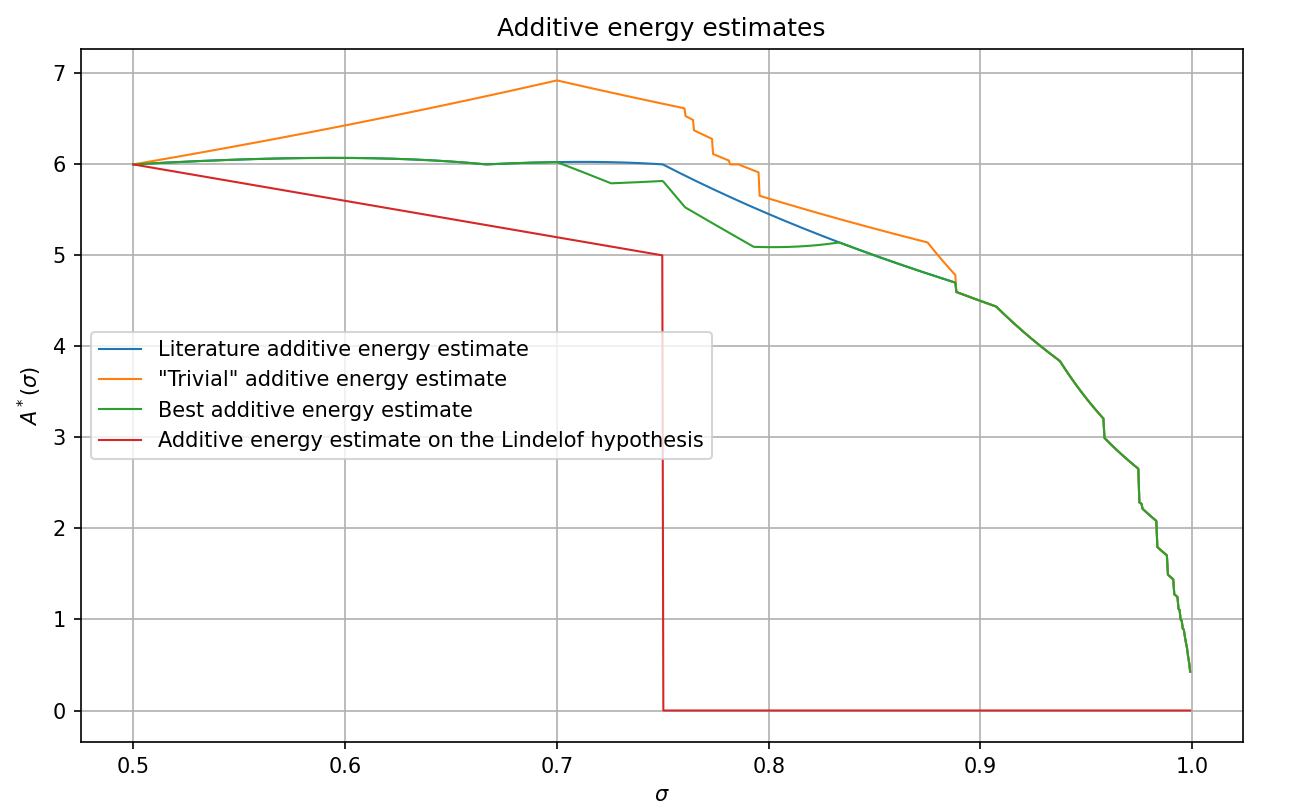
\includegraphics[width=0.5\textwidth]{chapter/zero_density_energy_estimate.png}
    \caption{Comparison of bounds on $\A^*(\sigma)$ under various assumptions.}
    \label{fig:zero_density_energy_estimate}
\end{figure}